\section{Konzept}

\subsection{Kontextdiagramm}
\begin{figure}[H]
  \begin{center}
    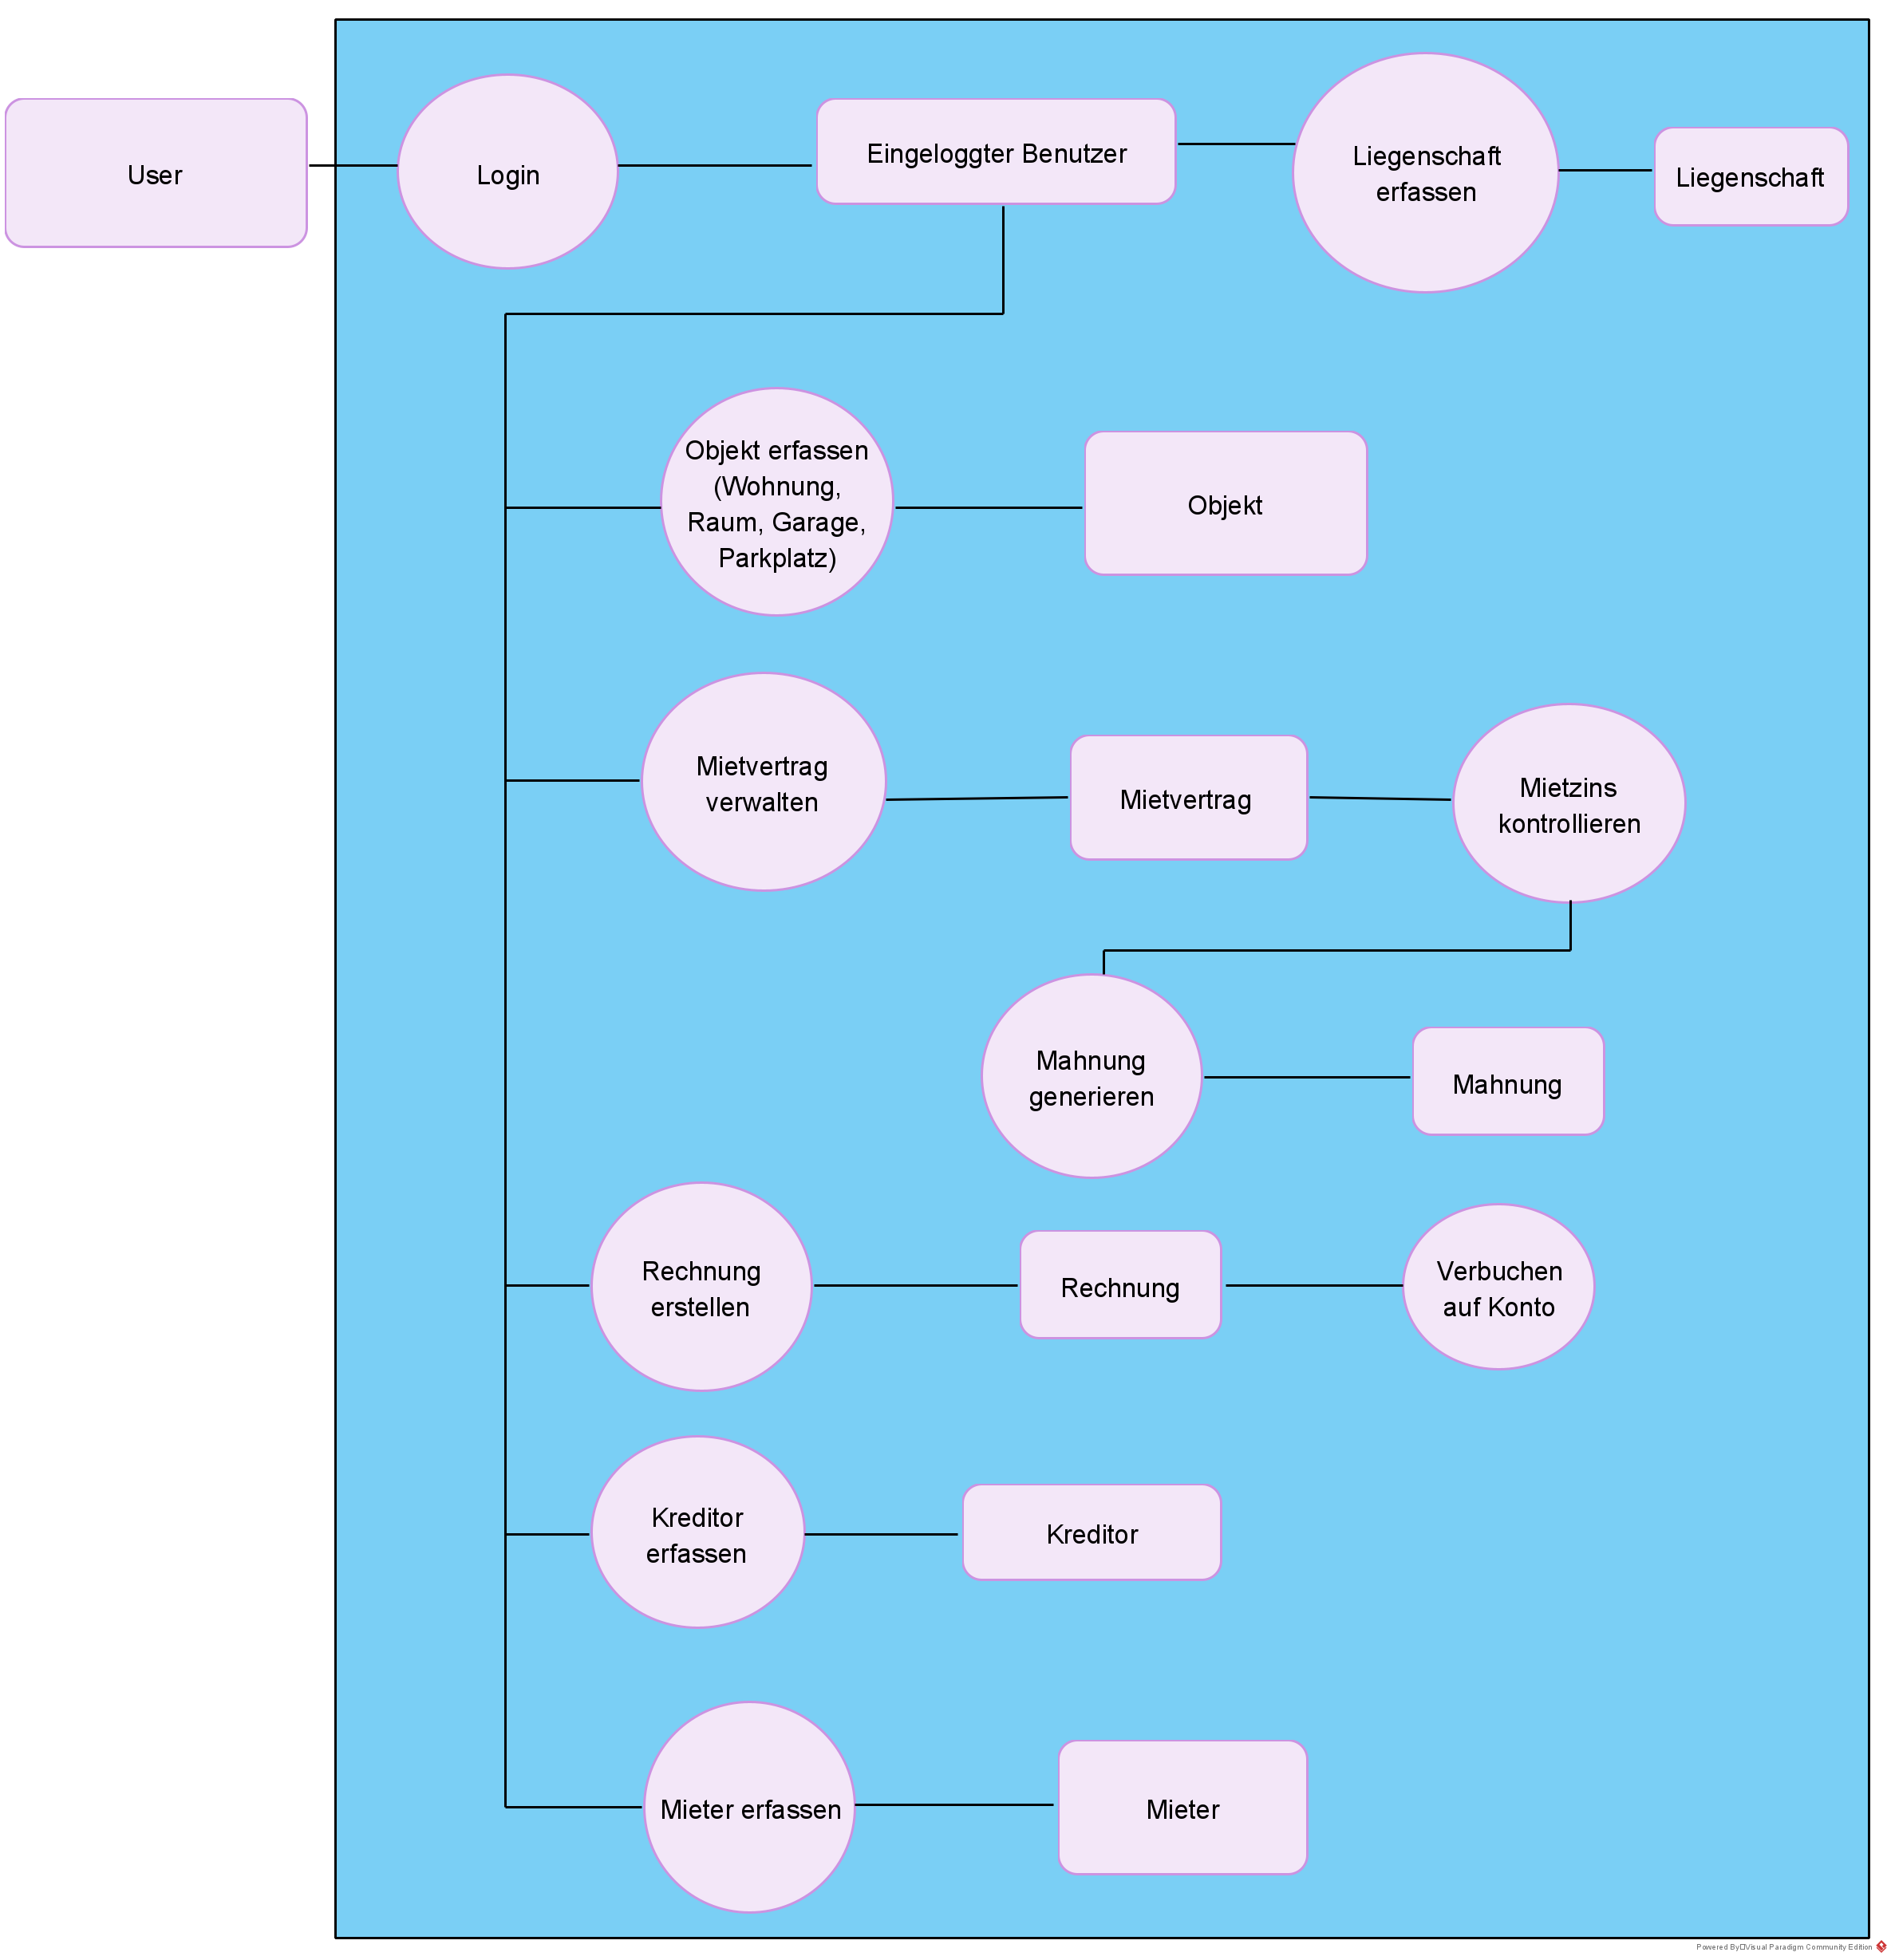
\includegraphics[width=0.99\linewidth]{content/diagrams/out/contextdiagram/context.png}
    \caption{Kontextdiagramm}
  \end{center}
  \label{contextdiag}
\end{figure}

\subsection{Geschäftsprozesse}
\begin{table}[H]
  \newcolumntype{a}{>{\columncolor[HTML]{4473C5}}L}
  \centering
  \settowidth\tymin{\textbf{Kurzbeschreibung}}
  \setlength\extrarowheight{2pt}
  \begin{tabulary}{1.0\textwidth}{|a|m{12cm}|}
    \hline
    \textbf{Name}& Verwaltung von Mietobjekten \\
    \hline 
    \textbf{Kurzbeschreibung} & Alle Geschäftsanwendungsfälle die nötig sid um Mietobjekte korrekt verwalten zu können und im Aufgabenbereich von ImmoGlobal liegen\\
    \hline
    \textbf{Geschäftsanwendungsfälle} & 
    \begin{itemize}
      \item Verwaltung von Objekten
      \item Verwaltung von Liegenschaften
      \item Übernahme- und Übergabeprotokoll der Mietobjekte
      \item Verwaltung der Mieter:innen
      \item Erstellen / Verwalten der Mietverträge
      \item Erfassen von Ein- und Ausgaben  (Mietzins, Nebenkosten, Gebühren für Unterhalt der Liegenschaft, etc.)
      \item Mietzins- und Nebenkostenkontrolle
      \item Rechnung erstellen
    \end{itemize}\\
    \hline
    \textbf{Verantwortlichkeit} & Geschäftsleiter\\
    \hline
    \textbf{Beteiligte} & 
    \begin{itemize}
      \item Mitarbeiter der Administration
      \item Hauswartungspersonen
      \item Mieter
    \end{itemize}\\
    \hline
  \end{tabulary}
  \caption{Geschäftsprozesse}
\end{table}


\subsection{Geschäftsanwendungsfälle}
\begin{table}[H]
  \newcolumntype{a}{>{\columncolor[HTML]{4473C5}}L}
  \centering
  \settowidth\tymin{\textbf{Kurzbeschreibung}}
  \setlength\extrarowheight{2pt}
  \begin{tabulary}{1.0\textwidth}{|a|m{12cm}|}
    \hline
    \textbf{Name}& Verwaltung von Objekten\\
    \hline 
    \textbf{Kurzbeschreibung} & Eine bestehendes Objekt muss editiert werden oder eine neues Objekt soll hinzugefügt werden \\
    \hline
    \textbf{Akteure} & Mitarbeiter in der Liegenschaftsverwaltung\\
    \hline
    \textbf{Auslöser} & Für die erfasste Liegenschaft wurden noch keine Objekte hinzugefügt\newline 
    Ein bestehendes Objekt muss ergänzt/korrigiert werden\\
    \hline
    \textbf{Ergebnis} & Das veränderte oder neu erstellte Objekt kann zu einer Liegenschaft hinzugefügt werden\\
    \hline
    \textbf{Eingehende Daten} & Informationen zum erfassenden Objekt\\
    \hline
    \textbf{Vorbedingungen} & Keine\\
    \hline
    \textbf{Nachbedingungen} & Keine\\
    \hline
    \textbf{Ablauf} & Der Benutzer trägt alle Muss-Daten für das neue Objekt ein und speichert es ab. \\
    \hline
  \end{tabulary}
  \caption{GA-Verwaltung von Objekten}
\end{table}

\begin{table}[H]
  \newcolumntype{a}{>{\columncolor[HTML]{4473C5}}L}
  \centering
  \settowidth\tymin{\textbf{Kurzbeschreibung}}
  \setlength\extrarowheight{2pt}
  \begin{tabulary}{1.0\textwidth}{|a|m{12cm}|}
    \hline
    \textbf{Name}& Verwaltung von Liegenschaften\\
    \hline 
    \textbf{Kurzbeschreibung} & Eine bestehende Liegenschaft muss editiert werden oder eine neue Liegenschaft soll hinzugefügt werden\\
    \hline
    \textbf{Akteure} & Mitarbeiter in der Liegenschaftsverwaltung\\
    \hline
    \textbf{Auslöser} & Die Verwaltung wird mit dem verwalten einer neuen Liegenschaft beauftragt \newline
    Bei einer Liegenschaft müssen Änderungen vorgenommen werden\\
    \hline
    \textbf{Ergebnis} & Die neuen Daten zu der Liegenschaft werden abgespeichert und in der Übersicht dargestellt\\
    \hline
    \textbf{Eingehende Daten} & Liegenschaft mit allen dazu gehörigen Informationen\\
    \hline
    \textbf{Vorbedingungen} & Die Daten zur Liegenschaft müssen bekannt sein\\
    \hline
    \textbf{Nachbedingungen} & Keine\\
    \hline
    \textbf{Ablauf} & Der Eingeloggte Mitarbeiter trägt alle Muss-Daten für die neue Liegenschaft ein und speichert diese. \newline
    Beim editieren einer Liegenschaft wird eine Vorhandene Liegenschaft bearbeitet.\\
    \hline
  \end{tabulary}
  \caption{GA-Verwaltung von Liegenschaften}
\end{table}

\begin{table}[H]
  \newcolumntype{a}{>{\columncolor[HTML]{4473C5}}L}
  \centering
  \settowidth\tymin{\textbf{Kurzbeschreibung}}
  \setlength\extrarowheight{2pt}
  \begin{tabulary}{1.0\textwidth}{|a|m{12cm}|}
    \hline
    \textbf{Name}& Übernahme- und Übergabeprotokoll der Mietobjekte\\
    \hline 
    \textbf{Kurzbeschreibung} & Bei Mietantritt wird ein Übernahmeprotokoll und bei Mietende wird ein Übergabeprotokoll erstellt\\
    \hline
    \textbf{Akteure} & Mitarbeiter in der Liegenschaftsverwaltung, Hauswartungsperson, Mieter\\
    \hline
    \textbf{Auslöser} & Beginn- oder Ende eines Mietverhältnisses\\
    \hline
    \textbf{Ergebnis} & Ein Übernahme- und Übergabeprotokoll für das Mietobjekt\\
    \hline
    \textbf{Eingehende Daten} &  
      $\bullet$ Kündigung \newline
      $\bullet$ Mietvertrag \newline
      $\bullet$ Bei Übergabe zurück an die Verwaltung das Übernahmeprotokoll\\
    \hline
    \textbf{Vorbedingungen} & Keine\\
    \hline
    \textbf{Nachbedingungen} & Keine\\
    \hline
    \textbf{Ablauf} & Für die Übernahme und die Übergabe wird von dem zuständigen Mitarbeiter das Protokoll ausgefüllt und von den Mietparteien auf Vollständigkeit geprüft und unterschrieben. Der Prozess findet komplett Digital statt. Unterschrieben wird das Protokoll auf einem unterschriftsfähigen Tablet. Anschliessend wird daraus ein PDF (PDF/A) generiert und dem Mieter wahlweise per E-Mail oder ausgedruckt per Post zugesandt\\
    \hline
  \end{tabulary}
  \caption{GA-Übernahme- und Übergabeprotokoll der Mietobjekte}
\end{table}

\begin{table}[H]
  \newcolumntype{a}{>{\columncolor[HTML]{4473C5}}L}
  \centering
  \settowidth\tymin{\textbf{Kurzbeschreibung}}
  \setlength\extrarowheight{2pt}
  \begin{tabulary}{1.0\textwidth}{|a|m{12cm}|}
    \hline
    \textbf{Name}& Verwaltung der Mieter:innen\\
    \hline 
    \textbf{Kurzbeschreibung} & Neue Mieter:innen werden in der Applikation hinzugefügt oder bestehende Mieter:innen bearbeitet\\
    \hline
    \textbf{Akteure} & Mitarbeiter in der Liegenschaftsverwaltung, Mieter\\
    \hline
    \textbf{Auslöser} & 
      $\bullet$ Vermietung eines Objektes an einen neuen Mieter:in \newline
      $\bullet$ Namensänderungen \newline
      $\bullet$ Zivilstandänderungen \newline
      $\bullet$ Geburten\\
    \hline
    \textbf{Ergebnis} &
      $\bullet$ Ein neuer Mieter:in wurde in der Applikation erfasst \newline
      $\bullet$ Änderung an bestehendem Mieter:in wurden durchgeführt\\
    \hline
    \textbf{Eingehende Daten} & Informationen über den Mieter:in\\
    \hline
    \textbf{Vorbedingungen} & Die Informationen über den Mieter:in müssen bekannt sein\\
    \hline
    \textbf{Nachbedingungen} & Keine\\
    \hline
    \textbf{Ablauf} & Der Benutzer der Applikation erstellt einen neuen Mieter:in. Er gibt alle Informationen ein und Speichert die Daten ab. Bei einer Änderung eines bestehenden Mieter:in, wird dieser in der Applikation gesucht und ausgewählt, editiert und abgespeichert\\
    \hline
  \end{tabulary}
  \caption{GA-Verwaltung der Mieter:innen}
\end{table}

\begin{table}[H]
  \newcolumntype{a}{>{\columncolor[HTML]{4473C5}}L}
  \centering
  \settowidth\tymin{\textbf{Kurzbeschreibung}}
  \setlength\extrarowheight{2pt}
  \begin{tabulary}{1.0\textwidth}{|a|m{12cm}|}
    \hline
    \textbf{Name}& Erstellen / Verwalten der Mietverträge\\
    \hline 
    \textbf{Kurzbeschreibung} & \\
    \hline
    \textbf{Akteure} & Mitarbeiter in der Liegenschaftsverwaltung, Mieter:in\\
    \hline
    \textbf{Auslöser} & Bewerbung eines neuen Mieters wurde akzeptiert\\
    \hline
    \textbf{Ergebnis} & Gültiger (unterschriebener) Mietvertrag\\
    \hline
    \textbf{Eingehende Daten} & 
      $\bullet$ Bewerbung mit allen Daten zum zukünftigen Mieter \newline
      $\bullet$ Betreibungsregisterauszug\\
    \hline
    \textbf{Vorbedingungen} & 
      $\bullet$ Bewerbung des Mieters wurde akzeptiert \newline
      $\bullet$ Bonität des Mieters wurde überprüft\\
    \hline
    \textbf{Nachbedingungen} & Keine\\
    \hline
    \textbf{Ablauf} & Der Benutzer der Applikation erstellt im betreffenden Mietobjekt einen neuen Mietvertrag. Den Mieter wählt er aus der Liste der vorhandenen Mieter aus. Falls der neue Mieter noch nicht erfasst wurde, kann er diesen erstellen. Anschliessend wird der neue Mietvertrag ausgedruckt und kann von beiden Parteien unterschrieben werden. Nachdem der Mietvertrag unterschrieben ist, wird dieser als PDF in der Applikation abgelegt und als Gültig markiert. Bei einer Kündigung des Mietverhältnisses wird die Kündigung des Mietvertrags in die Applikation hochgeladen und der der Status auf gekündigt geändert. Sobald dann das ende des Mietverhältnisses erreicht ist, wird der Status auf beendet gesetzt.\\
    \hline
  \end{tabulary}
  \caption{GA-Erstellen / Verwalten der Mietverträge}
\end{table}

\begin{table}[H]
  \newcolumntype{a}{>{\columncolor[HTML]{4473C5}}L}
  \centering
  \settowidth\tymin{\textbf{Kurzbeschreibung}}
  \setlength\extrarowheight{2pt}
  \begin{tabulary}{1.0\textwidth}{|a|m{12cm}|}
    \hline
    \textbf{Name}& Erfassen von Ein- und Ausgaben\\
    \hline 
    \textbf{Kurzbeschreibung} & Alle Einnahmen und alle Ausgaben werden erfasst\\
    \hline
    \textbf{Akteure} & Mitarbeiter in der Liegenschaftsverwaltung\\
    \hline
    \textbf{Auslöser} & Zahlungs-Eingang / Ausgang\\
    \hline
    \textbf{Ergebnis} & Neuer Zahlungs-Ein/Ausgang ist im System erfasst\\
    \hline
    \textbf{Eingehende Daten} &
      $\bullet$ Rechnungen \newline
      $\bullet$ Abrechnungen\\
    \hline
    \textbf{Vorbedingungen} & Keine\\
    \hline
    \textbf{Nachbedingungen} & Keine\\
    \hline
    \textbf{Ablauf} & Der Benutzer trägt alle Zahlungseingänge im System ein. Wenn eine Zahlung anhand einer Rechnung getätigt werden muss, bezahlt er diese und trägt den Rechnungsbetrag ebenfalls im System ein\\
    \hline
  \end{tabulary}
  \caption{GA-Kreditor erfassen}
\end{table}

\begin{table}[H]
  \newcolumntype{a}{>{\columncolor[HTML]{4473C5}}L}
  \centering
  \settowidth\tymin{\textbf{Kurzbeschreibung}}
  \setlength\extrarowheight{2pt}
  \begin{tabulary}{1.0\textwidth}{|a|m{12cm}|}
    \hline
    \textbf{Name}&Mietzins- und Nebenkostenkontrolle\\
    \hline 
    \textbf{Kurzbeschreibung} & Der Eingang der Mietzinse und der Nebenkostenzahlungen wird kontrolliert und bei fehlenden Eingängen wird eine Mahnung erstellt\\
    \hline
    \textbf{Akteure} & Mitarbeiter in der Liegenschaftsverwaltung\\
    \hline
    \textbf{Auslöser} & Mietzins- und Nebenkostenzahlungsüberprüfung\\
    \hline
    \textbf{Ergebnis} & Bei negativer Prüfung eine Mahnung\newline 
    Bei positiver Prüfung nichts\\
    \hline
    \textbf{Eingehende Daten} & Mietvertrag\\
    \hline
    \textbf{Vorbedingungen} & Es müssen gültige Mietverträge im System erfasst sein \\
    \hline
    \textbf{Nachbedingungen} & Keine \\
    \hline
    \textbf{Ablauf} & Der Benutzer überprüft, ob für ein entsprechendes Objekt die Miete und die Nebenkosten bezahlt wurden. Wenn die Miete oder die Nebenkosten noch nicht bezahlt wurden, kann er eine Mahnung generieren und ausdrucken.\\
    \hline
  \end{tabulary}
  \caption{GA-Mietzins- und Nebenkostenkontrolle}
\end{table}

\begin{table}[H]
  \newcolumntype{a}{>{\columncolor[HTML]{4473C5}}L}
  \centering
  \settowidth\tymin{\textbf{Kurzbeschreibung}}
  \setlength\extrarowheight{2pt}
  \begin{tabulary}{1.0\textwidth}{|a|m{12cm}|}
    \hline
    \textbf{Name}&Rechnung erstellen\\
    \hline 
    \textbf{Kurzbeschreibung} & Eine neue Rechnung erstellen\\
    \hline
    \textbf{Akteure} & Mitarbeiter in der Liegenschaftsverwaltung\\
    \hline
    \textbf{Auslöser} & Es wurde eine Dienstleistung, die die Liegenschaftsverwaltung getätigt hat, bezogen \newline 
    Für eine Liegenschaft oder ein Objekt wurde die Nebenkostenabrechnung erstellt\\
    \hline
    \textbf{Ergebnis} & Eine Rechnung die nach dem freigeben nicht mehr bearbeitet werden kann\\
    \hline
    \textbf{Eingehende Daten} & Informationen warum die Rechnung erstellt werden muss \\
    \hline
    \textbf{Vorbedingungen} & Keine\\
    \hline
    \textbf{Nachbedingungen} & Keine\\
    \hline
    \textbf{Ablauf} & Der Benutzer erstellt eine neue Rechnung und gibt alle nötigen Informationen für die Rechnung ein. Der Benutzer ordnet die Rechnung einem bestimmten Konto zu. Falls das Konto noch nicht besteht, muss dieses zuerst noch erstellt werden. Wenn die Rechnung für den Kreditor/Mieter freigegeben wird, ändert der Status der Rechnung auf ''freigeben'' und kann nicht mehr abgeändert werden. Wenn nach der Freigabe Fehler bemerkt werden, muss der Status der Rechnung auf Storniert gewechselt werden und eine neue Rechnung erstellt werden. Der Benutzer hat aber auch die Möglichkeit, die Rechnung nicht freizugeben und die Bearbeitung zu einem späteren Zeitpunkt fortzusetzen.\\
    \hline
  \end{tabulary}
  \caption{GA-Rechnung erstellen}
  \label{GA-rechnungErstellen}
\end{table}
\newpage
\subsection{Use-Case-Beschreibungen}

\begin{figure}[H]
  \begin{center}
    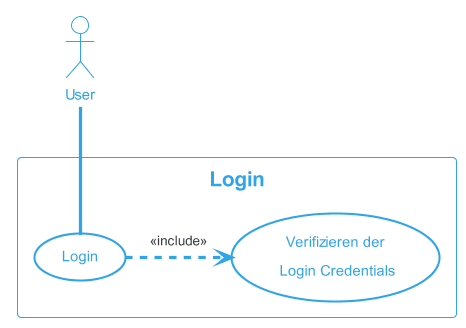
\includegraphics[width=0.6\linewidth]{content/diagrams/out/usecase/login/Login.png}
    \caption{UC-Login}
    \label{login}
  \end{center}
\end{figure}

\begin{table}[H]
  \newcolumntype{a}{>{\columncolor[HTML]{4473C5}}L}
  \centering
  \settowidth\tymin{\textbf{Kurzbeschreibung}}
  \setlength\extrarowheight{2pt}
  \begin{tabulary}{1.0\textwidth}{|a|m{14cm}|}
    \hline
    \textbf{Name}& Login\\
    \hline
    \textbf{Akteur}& Mitarbeiter:in der Liegenschaftsverwaltung, Hauswartungspersonen, Geschäftsführer\\
    \hline 
    \textbf{Beschreibung} & Ein Akteur will sich in der Applikation anmelden\\
    \hline
    \textbf{Daten} & Login-Daten des Benutzers\\
    \hline
    \textbf{Auslöser} & Benutzerbefehl der von dem entsprechenden Akteur initiiert wird\\
    \hline
    \textbf{Antwort} & Bestätigung, dass das Login erfolgreich war\\
    \hline
    \textbf{Kommentare} & -\\
    \hline
  \end{tabulary}
  \caption{UC-Login}
\end{table}

\begin{figure}[H]
  \begin{center}
    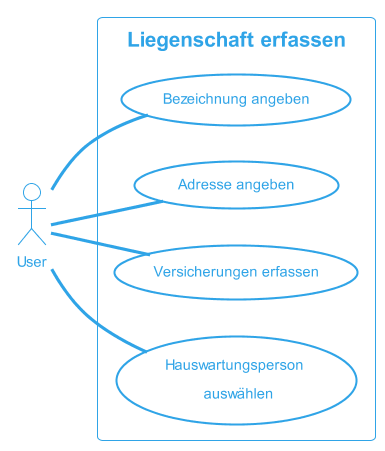
\includegraphics[width=0.43\linewidth]{content/diagrams/out/usecase/liegenschaftErfassen/LiegenschaftErfassen.png}
    \caption{UC-Liegenschaft erfassen}
    \label{Liegenschaft}
  \end{center}
\end{figure}

\vspace*{-1cm}

\begin{table}[H]
  \newcolumntype{a}{>{\columncolor[HTML]{4473C5}}L}
  \centering
  \settowidth\tymin{\textbf{Kurzbeschreibung}}
  \setlength\extrarowheight{2pt}
  \begin{tabulary}{1.0\textwidth}{|a|m{14cm}|}
    \hline
    \textbf{Name}& Liegenschaft erfassen\\
    \hline
    \textbf{Akteur}& Mitarbeiter:in der Liegenschaftsverwaltung\\
    \hline 
    \textbf{Beschreibung} & Der zuständige Mitarbeiter:in loggt sich in der Applikation ein und kann anschliessend die Liegenschaft über einen Button erfassen. Es müssen alle Daten zur Liegenschaft eingetragen werden sonst kann der Mitarbeiter die Liegenschaft nicht abspeichern.\\
    \hline
    \textbf{Daten} & Informationen zur Liegenschaft\\
    \hline
    \textbf{Auslöser} & Benutzerbefehl der von dem entsprechenden Akteur initiiert wird\\
    \hline
    \textbf{Antwort} & Bestätigung, dass das erfassen der Liegenschaft erfolgreich war\\
    \hline
    \textbf{Kommentare} & Bei fehlenden Angaben wird dem Benutzer eine Fehlermeldung angezeigt\\
    \hline
  \end{tabulary}
  \caption{UC-Liegenschaft erfassen}
\end{table}

\begin{figure}[H]
  \begin{center}
    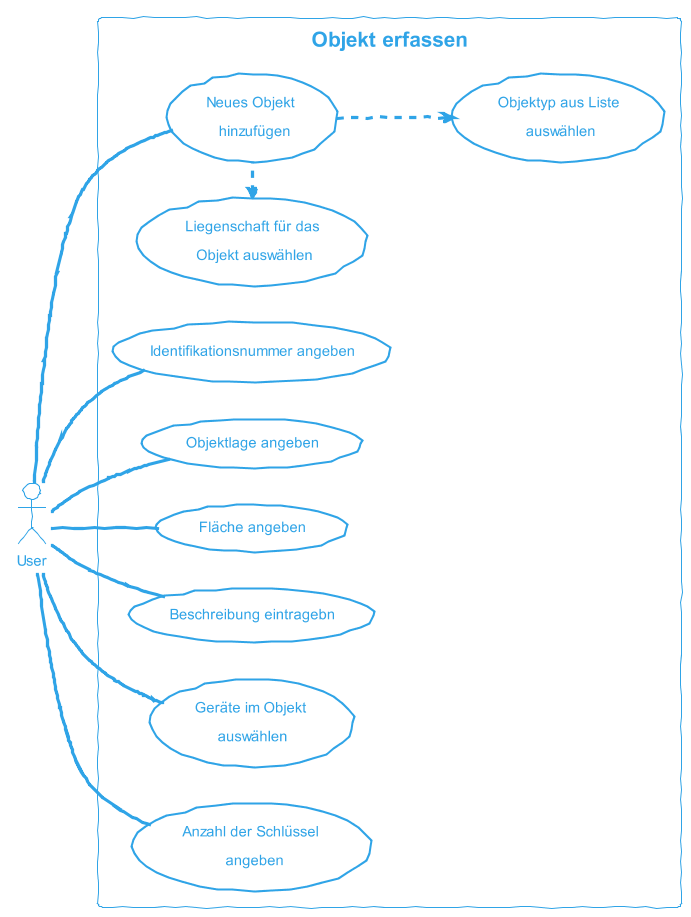
\includegraphics[width=0.8\linewidth]{content/diagrams/out/usecase/objektErfassen/ObjektErfassen.png}
    \caption{UC-Objekt erfassen}
    \label{objekt}
  \end{center}
\end{figure}

\vspace*{-1cm}

\begin{table}[H]
  \newcolumntype{a}{>{\columncolor[HTML]{4473C5}}L}
  \centering
  \settowidth\tymin{\textbf{Kurzbeschreibung}}
  \setlength\extrarowheight{2pt}
  \begin{tabulary}{1.0\textwidth}{|a|m{14cm}|}
    \hline
    \textbf{Name}& Objekt erfassen\\
    \hline
    \textbf{Akteur}& Mitarbeiter:in der Liegenschaftsverwaltung\\
    \hline 
    \textbf{Beschreibung} & Der zuständige Mitarbeiter:in loggt sich in der Applikation ein und kann anschliessend das Objekt über einen Button erfassen. Es müssen alle Daten zum Objekt eingetragen werden sonst kann dieses nicht abgespeichert werden\\
    \hline
    \textbf{Daten} & Informationen zum Objekt\\
    \hline
    \textbf{Auslöser} & Benutzerbefehl der von dem entsprechenden Akteur initiiert wird\\
    \hline
    \textbf{Antwort} & Bestätigung, dass das erfassen des Objektes erfolgreich war\\
    \hline
    \textbf{Kommentare} & Bei fehlenden Angaben wird dem Benutzer eine Fehlermeldung angezeigt\newline 
    Ein Objekt kann nur über eine Liegenschaft erfasst werden\\
    \hline
  \end{tabulary}
  \caption{UC-Objekt erfassen}
\end{table}

\begin{figure}[H]
  \begin{center}
    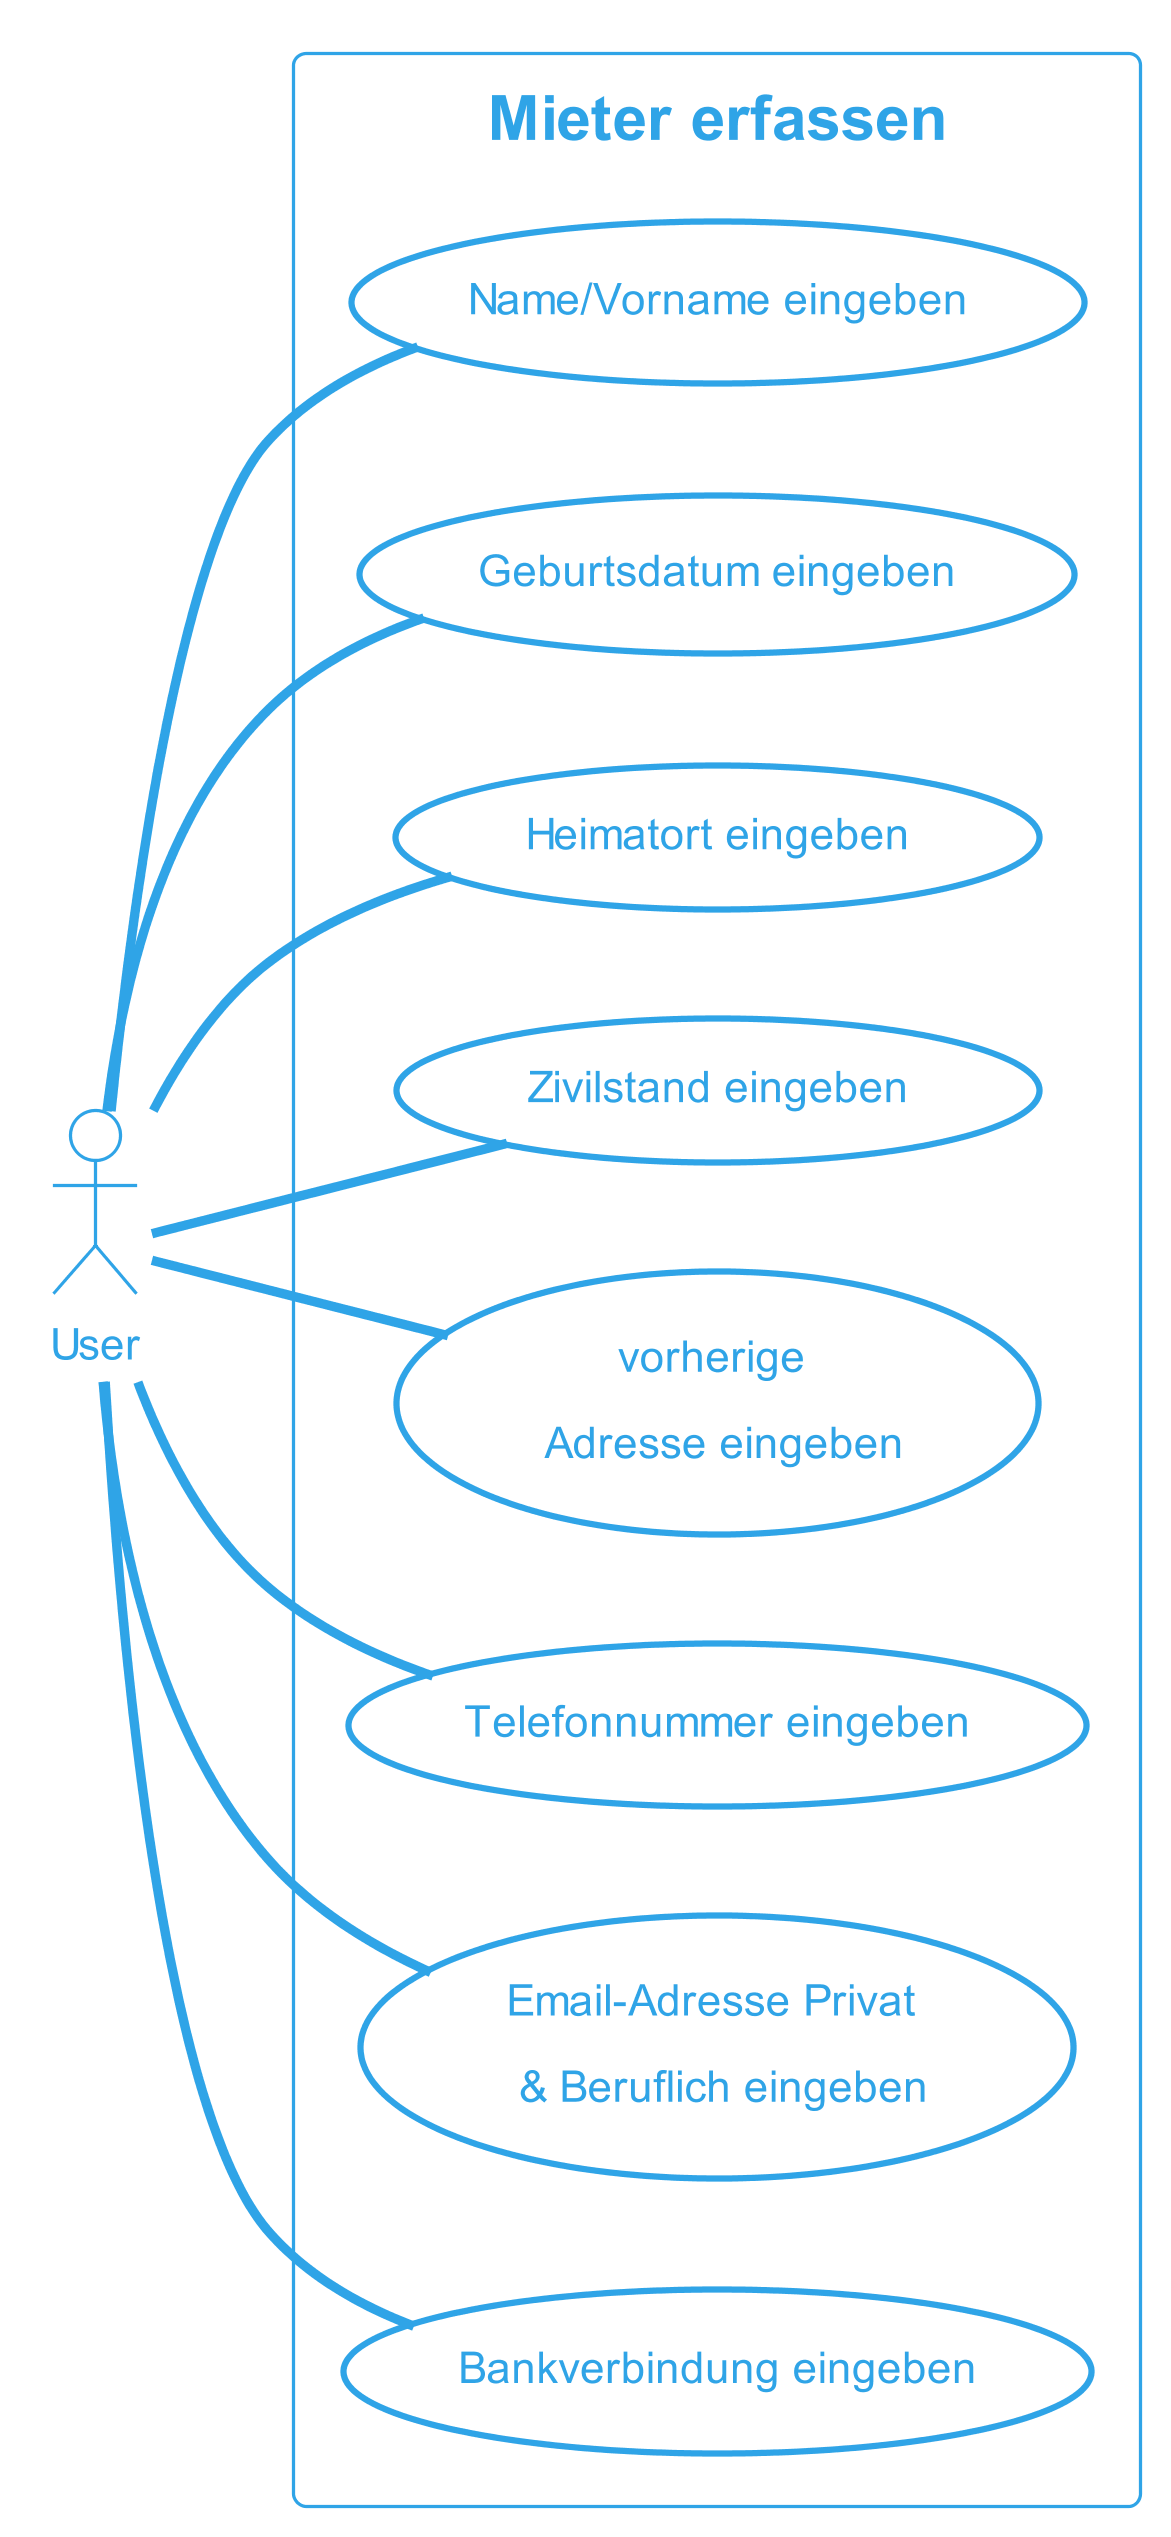
\includegraphics[width=0.4\linewidth]{content/diagrams/out/usecase/mieterErfassen/Mieter erfassen.png}
    \caption{UC-Mieter:in erfassen}
    \label{mieterErfassen}
  \end{center}
\end{figure}

\begin{table}[H]
  \newcolumntype{a}{>{\columncolor[HTML]{4473C5}}L}
  \centering
  \settowidth\tymin{\textbf{Kurzbeschreibung}}
  \setlength\extrarowheight{2pt}
  \begin{tabulary}{1.0\textwidth}{|a|m{14cm}|}
    \hline
    \textbf{Name}& Mieter:in erfassen\\
    \hline
    \textbf{Akteur}& Mitarbeiter:in der Liegenschaftsverwaltung\\
    \hline 
    \textbf{Beschreibung} & Wird die Bewerbung eines Mieters für ein Objekt angenommen, muss dieser Mieter:in in der Applikation erfasst werden. Der zuständige Mitarbeiter:in loggt sich dazu in der Applikation ein und kann den Mieter:in im entsprechenden Formular erfassen\\
    \hline
    \textbf{Daten} & Vollständige Daten zum Mieter\\
    \hline
    \textbf{Auslöser} & Benutzerbefehl der von dem entsprechenden Akteur initiiert wird\\
    \hline
    \textbf{Antwort} & Bestätigung, dass der Mieter erfolgreich erfasst wurde\\
    \hline
    \textbf{Kommentare} & -\\
    \hline
  \end{tabulary}
  \caption{UC-Mieter:in erfassen}
\end{table}

\begin{figure}[H]
  \begin{center}
    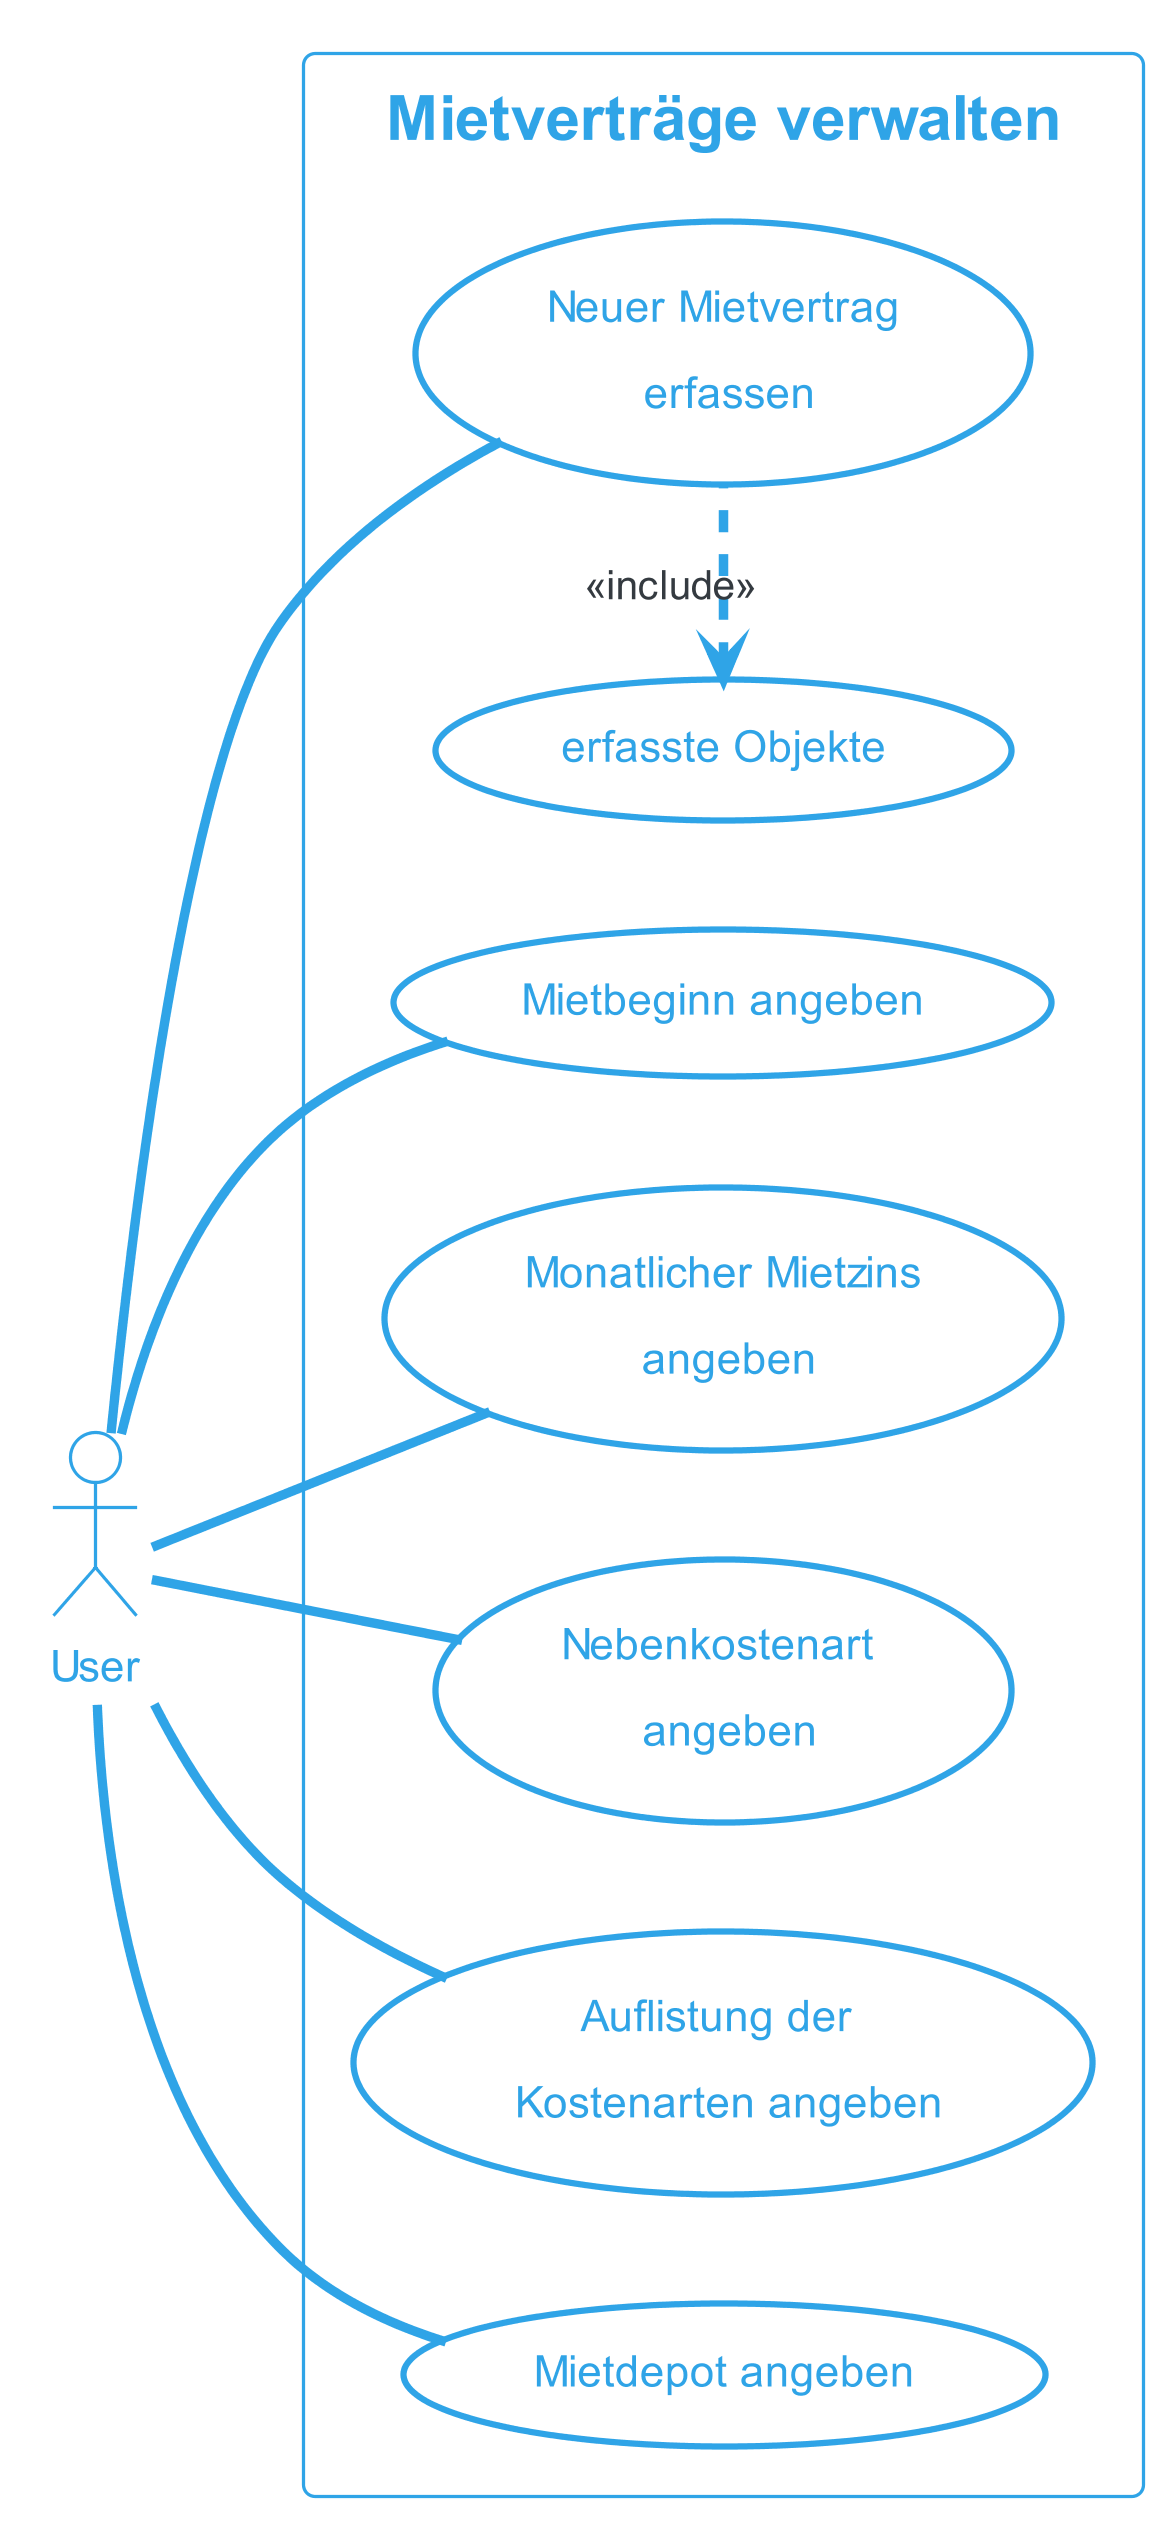
\includegraphics[width=0.43\linewidth]{content/diagrams/out/usecase/mietverträgeVerwalten/MietverträgeVerwalten.png}
    \caption{UC-Mietverträge verwalten}
    \label{MietvertraegeVerwalten}
  \end{center}
\end{figure}

\vspace*{-1cm}

  \begin{table}[H]
    \newcolumntype{a}{>{\columncolor[HTML]{4473C5}}L}
    \centering
    \settowidth\tymin{\textbf{Kurzbeschreibung}}
    \setlength\extrarowheight{2pt}
      \begin{tabulary}{1.0\textwidth}{|a|m{14cm}|}
        \hline
        \textbf{Name}& Mietverträge verwalten\\
      \hline
      \textbf{Akteur}& Mitarbeiter:in der Liegenschaftsverwaltung\\
      \hline 
      \textbf{Beschreibung} & Der zuständige Mitarbeiter:in loggt sich in der Applikation ein und erstellt anschliessend einen neuen Mietvertrag der noch den Status ungültig hat, bis dieser von beiden Parteien unterschrieben wurde\\
      \hline
      \textbf{Daten} & Alle Daten die zum erfassen des Mietvertrags nötig sind \\
      \hline
      \textbf{Auslöser} & Benutzerbefehl der von dem entsprechenden Akteur initiiert wird\\
      \hline
      \textbf{Antwort} & Bestätigung, dass der Mietvertrag erfolgreich erfasst wurde und ausgedruckt werden kann\\
      \hline
      \textbf{Kommentare} & Bei fehlenden Angaben wird dem Benutzer eine Fehlermeldung angezeigt\\
      \hline
  \end{tabulary}
  \caption{UC-Mietverträge verwalten}
  \end{table}

\begin{figure}[H]
  \begin{center}
    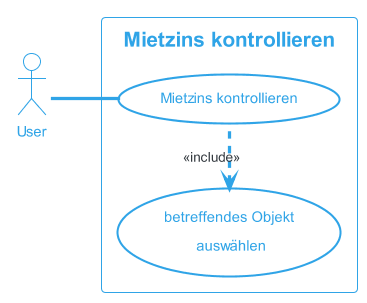
\includegraphics[width=0.4\linewidth]{content/diagrams/out/usecase/mietzinsKontrollieren/MietzinsKontrollieren.png}
    \caption{UC-Mietzins kontrollieren}
    \label{MietzinsKontrollieren}
  \end{center}
\end{figure}

\begin{table}[H]
  \newcolumntype{a}{>{\columncolor[HTML]{4473C5}}L}
  \centering
  \settowidth\tymin{\textbf{Kurzbeschreibung}}
  \setlength\extrarowheight{2pt}
  \begin{tabulary}{1.0\textwidth}{|a|m{14cm}|}
    \hline
    \textbf{Name}& Mietzins kontrollieren\\
    \hline
    \textbf{Akteur}& Mitarbeiter:in der Liegenschaftsverwaltung\\
    \hline 
    \textbf{Beschreibung} & Wenn die Zahlungen geprüft werden müssen, loggt sich der zuständige Mitarbeiter:in ein und kann auf dem entsprechenden Objekt Kontrollieren ob die Miete oder die Nebenkosten schon als ''bezahlt'' markiert wurde\\
    \hline
    \textbf{Daten} & Zu prüfendes Objekt\\
    \hline
    \textbf{Auslöser} & Benutzerbefehl der von dem entsprechenden Akteur initiiert wird\\
    \hline
    \textbf{Antwort} & Zahlungen wurde getätigt oder im Verzug\\
    \hline
    \textbf{Kommentare} & Bei Zahlungen im Verzug wird der nächste UseCase \fref{mahnung} eingesetzt\\
    \hline
  \end{tabulary}
  \caption{UC-Mietzins kontrollieren}
\end{table}

\newpage

\begin{figure}[H]
  \begin{center}
    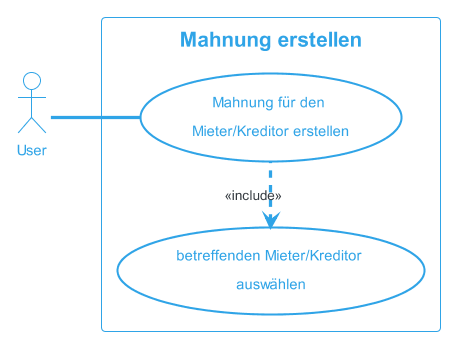
\includegraphics[width=0.5\linewidth]{content/diagrams/out/usecase/mahnungGenerieren/MahnungErstellen.png}
    \caption{UC-Mahnung erstellen}
    \label{mahnung}
  \end{center}
\end{figure}

\begin{table}[H]
  \newcolumntype{a}{>{\columncolor[HTML]{4473C5}}L}
  \centering
  \settowidth\tymin{\textbf{Kurzbeschreibung}}
  \setlength\extrarowheight{2pt}
  \begin{tabulary}{1.0\textwidth}{|a|m{14cm}|}
    \hline
    \textbf{Name}& Mahnung erstellen\\
    \hline
    \textbf{Akteur}& Mitarbeiter:in der Liegenschaftsverwaltung\\
    \hline 
    \textbf{Beschreibung} & Fällt die Prüfung der Mietzins-oder Nebenkostenzahlung negativ aus, kann der Benutzer eine Mahnung für den Mieter erstellen \\
    \hline
    \textbf{Daten} & Rechnungsbetrag\\
    \hline
    \textbf{Auslöser} & Benutzerbefehl der von dem entsprechenden Akteur initiiert wird\\
    \hline
    \textbf{Antwort} & Bestätigung, dass die Mahnung erfolgreich erstellt wurde und jetzt ausgedruckt werden kann\\
    \hline
    \textbf{Kommentare} & Normalerweise ist der zuständige Mitarbeiter:in in der Applikation schon eingeloggt da er die Prüfung der Zahlung vorgenommen hatte. Das erstellen der Mahnung wird dann direkt von dort aus ausgelöst\\
    \hline
  \end{tabulary}
  \caption{UC-Mahnung erstellen}
\end{table}

\begin{figure}[H]
  \begin{center}
    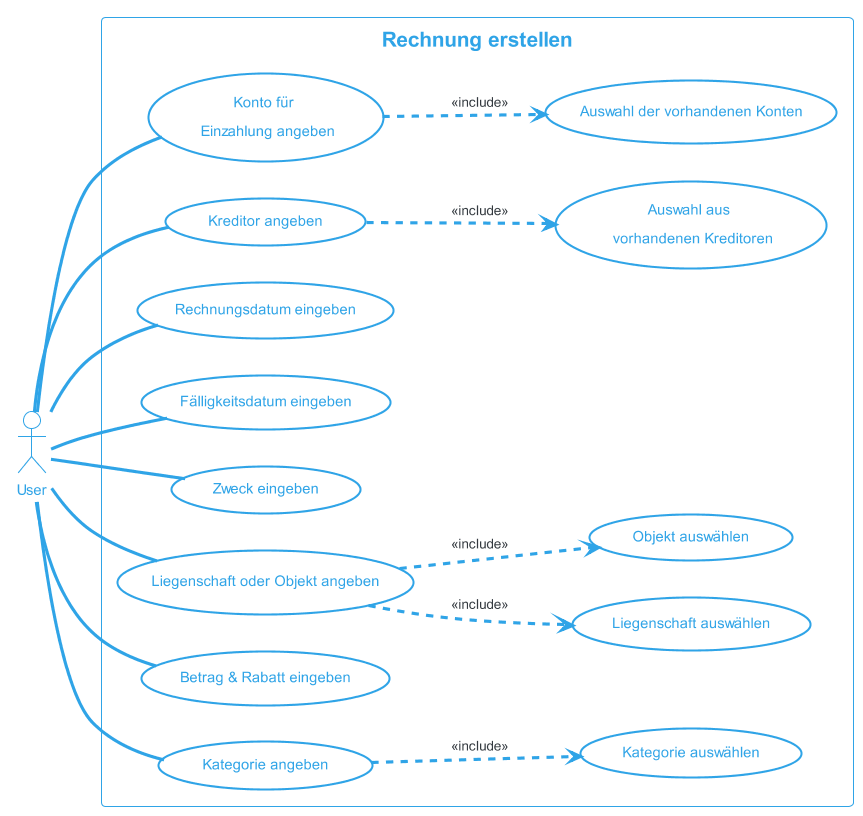
\includegraphics[width=0.85\linewidth]{content/diagrams/out/usecase/rechnungErstellen/Rechnung erstellen.png}
    \caption{UC-Rechnung erstellen}
    \label{RechnungErstellen}
  \end{center}
\end{figure}
\vspace*{-1.2cm}
\begin{table}[H]
  \newcolumntype{a}{>{\columncolor[HTML]{4473C5}}L}
  \centering
  \settowidth\tymin{\textbf{Kurzbeschreibung}}
  \setlength\extrarowheight{2pt}
  \begin{tabulary}{1.0\textwidth}{|a|m{14cm}|}
    \hline
    \textbf{Name}& Rechnung erstellen\\
    \hline
    \textbf{Akteur}& Mitarbeiter:in der Liegenschaftsverwaltung\\
    \hline 
    \textbf{Beschreibung} & Um eine Rechnung zu erstellen, muss sich der Zuständige Mitarbeiter:in in der Applikation einloggen. Es kann dann für eine Dienstleistung eine Rechnung erstellt werden. Um die Rechnung für eine Dienstleistung zu erstellen, müssen alle Daten eingegeben werden \newline 
    Wird eine Rechnung für die fällige Miete oder die Nebenkosten erstellt, werden die Daten für die Rechnung aus der angewählten Liegenschaft oder Objekt in die Rechnung eingefügt. Allfällige Anpassungen können nachträglichen als separate Rechnungsposition hinzugefügt werden \newline
    Die Rechnungen werden immer einem Konto zugeordnet. Falls das gewünschte Konto noch nicht besteht, muss es noch erstellt werden\\
    \hline
    \textbf{Daten} &       
      $\bullet$ Kreditor\newline
      $\bullet$ Rechnungsbetrag \newline
      $\bullet$ Objekt oder Liegenschaft\\
    \hline
    \textbf{Auslöser} & Benutzerbefehl der von dem entsprechenden Akteur initiiert wird\\
    \hline
    \textbf{Antwort} & Bestätigung, dass die Rechnung erfolgreich erstellt wurde und ausgedruckt werden kann\\
    \hline
    \textbf{Kommentare} & Falls der Kreditor oder das Konto noch nicht erfasst wurde, muss dies noch gemacht werden. Siehe UseCase \hyperref[kreditorErfassen]{Kreditor Erfassen \fref{kreditorErfassen}} bzw. \hyperref[kreditorErfassen]{Kreditor Erfassen \fref{kreditorErfassen}}\\
    \hline
  \end{tabulary}
  \caption{UC-Rechnung erstellen}
\end{table}

\begin{figure}[H]
  \begin{center}
      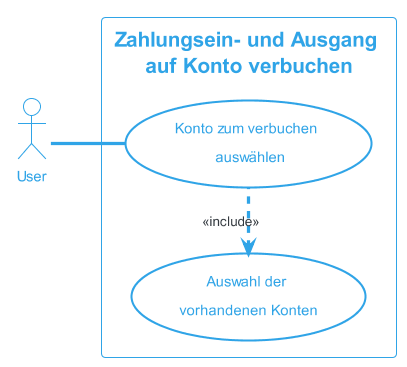
\includegraphics[width=0.5\linewidth]{content/diagrams/out/usecase/verbuchenAufKonto/ZahlungseingangaufKontoverbuchen.png}
    \caption{UC-Zahlungseingang auf Konto verbuchen}
    \label{ZahlungaufKonto}
  \end{center}
\end{figure}

\begin{table}[H]
  \newcolumntype{a}{>{\columncolor[HTML]{4473C5}}L}
  \centering
  \settowidth\tymin{\textbf{Kurzbeschreibung}}
  \setlength\extrarowheight{2pt}
  \begin{tabulary}{1.0\textwidth}{|a|m{14cm}|}
    \hline
    \textbf{Name}& Zahlungsein- und Ausgang auf Konto verbuchen\\
    \hline
    \textbf{Akteur}& Mitarbeiter:in der Liegenschaftsverwaltung\\
    \hline 
    \textbf{Beschreibung} & Bei einem Zahlungseingang, muss dieser auf ein entsprechendes Konto verbucht werden. Normalerweise gibt es aufgrund einer gestellten Rechnung einen Zahlungseingang. Wenn die Rechnung als bezahlt markiert wird, wird der Zahlungseingang auf das mit der Rechnung verknüpfte Konto verbucht \newline
    Falls es einen Zahlungsein- oder Ausgang gibt der nicht aufgrund einer Rechnung geschieht, muss dieser Eintrag manuell für das entsprechende Konto erstellt werden\\
    \hline
    \textbf{Daten} & Rechnungsnummer oder Zahlungsbetrag und Konto\\
    \hline
    \textbf{Auslöser} & Zahlungseingang\\
    \hline
    \textbf{Antwort} & Bestätigung, dass der Zahlungseingang verbucht wurde\\
    \hline
    \textbf{Kommentare} & Wenn das Konto zu dem der Zahlungsein- oder Ausgang erfasst werden soll noch nicht besteht, muss dies noch erstellt werden. Siehe \hyperref[kontoErstellen]{Konto erstellen \fref{kontoErstellen}}\\
    \hline
  \end{tabulary}
  \caption{UC-Zahlungsein- und Ausgang auf Konto verbuchen}
\end{table}

\newpage
\begin{figure}[H]
  \begin{center}
    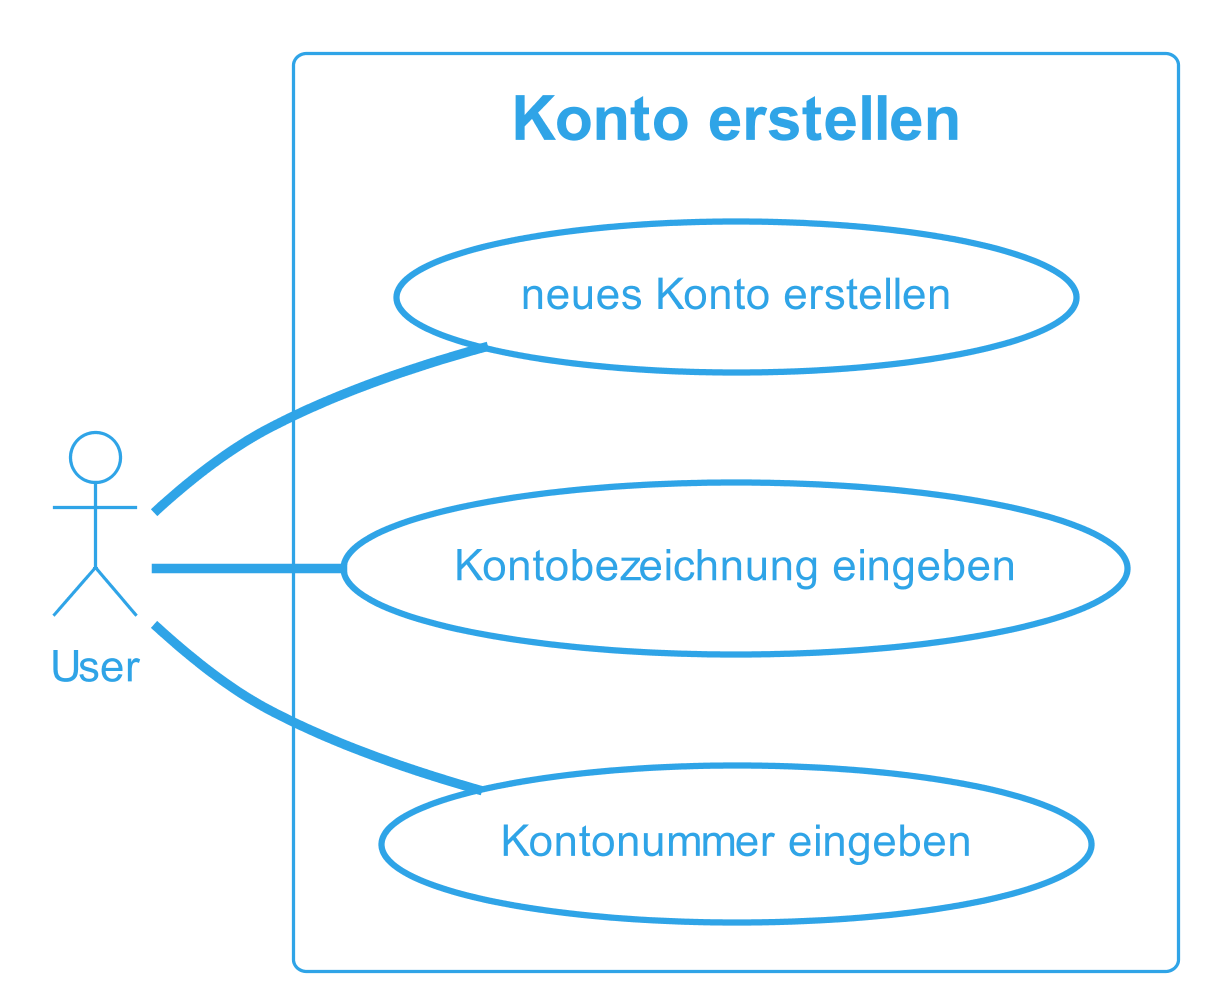
\includegraphics[width=0.5\linewidth]{content/diagrams/out/usecase/kontoErstellen/kontoErstellen.png}
    \caption{UC-Konto erstellen}
    \label{kontoErstellen}
  \end{center}
\end{figure}

\begin{table}[H]
  \newcolumntype{a}{>{\columncolor[HTML]{4473C5}}L}
  \centering
  \settowidth\tymin{\textbf{Kurzbeschreibung}}
  \setlength\extrarowheight{2pt}
  \begin{tabulary}{1.0\textwidth}{|a|m{14cm}|}
    \hline
    \textbf{Name}& Konto erstellen\\
    \hline
    \textbf{Akteur}& Mitarbeiter:in der Liegenschaftsverwaltung\\
    \hline 
    \textbf{Beschreibung} & Ein neues Konto zum verbuchen Der Zahlungen muss erstellt werden\\
    \hline
    \textbf{Daten} & Kontobezeichnung und Kontonummer\\
    \hline
    \textbf{Auslöser} & Benutzerbefehl, der von dem entsprechenden Akteur initiiert wird\\
    \hline
    \textbf{Antwort} & Bestätigung, dass das Konto erfolgreich erstellt wurde\\
    \hline
    \textbf{Kommentare} & -\\
    \hline
  \end{tabulary}
  \caption{UC-Konto erstellen}
\end{table}

\begin{figure}[H]
  \begin{center}
    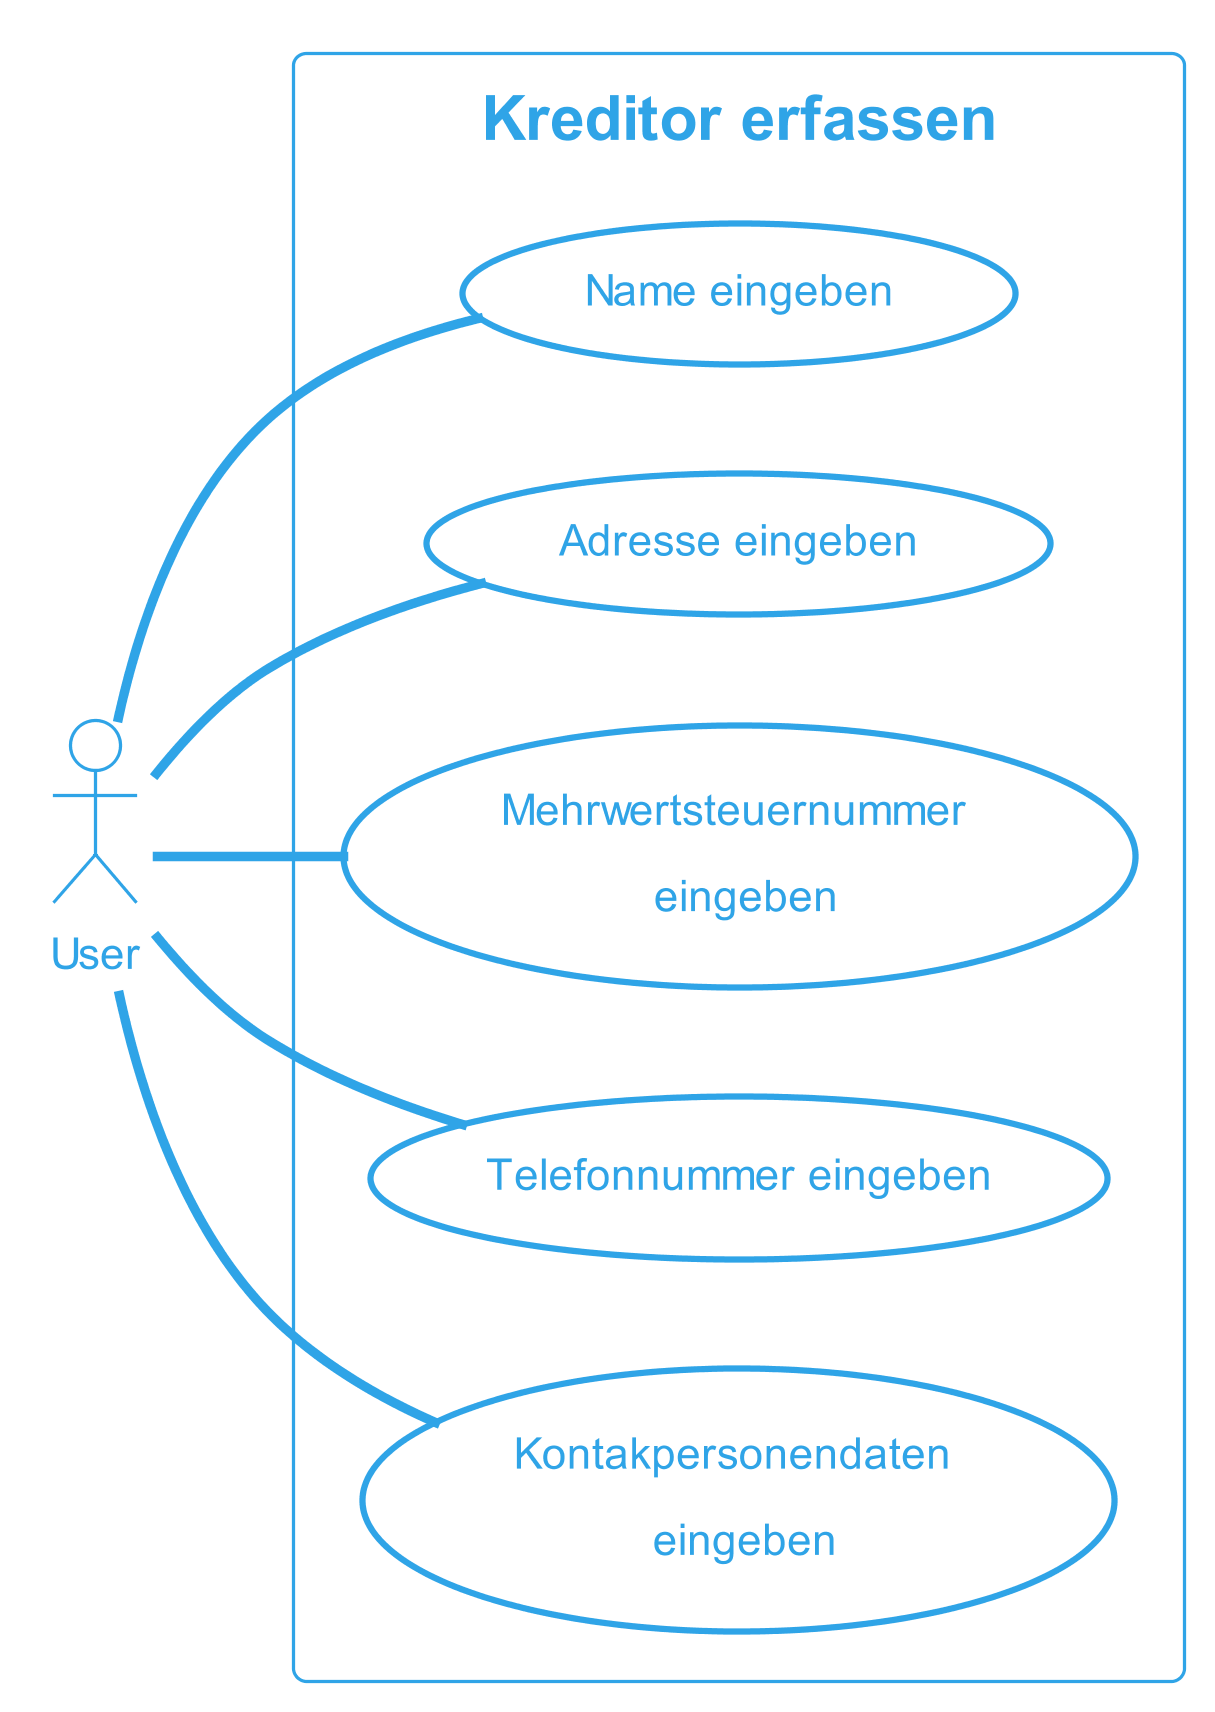
\includegraphics[width=0.5\linewidth]{content/diagrams/out/usecase/kreditorErfassen/Kreditor erfassen.png}
    \caption{UC-Kreditor erfassen}
    \label{kreditorErfassen}
  \end{center}
\end{figure}

\begin{table}[H]
  \newcolumntype{a}{>{\columncolor[HTML]{4473C5}}L}
  \centering
  \settowidth\tymin{\textbf{Kurzbeschreibung}}
  \setlength\extrarowheight{2pt}
  \begin{tabulary}{1.0\textwidth}{|a|m{14cm}|}
    \hline
    \textbf{Name}& Kreditor erfassen\\
    \hline
    \textbf{Akteur}& Mitarbeiter:in der Liegenschaftsverwaltung\\
    \hline 
    \textbf{Beschreibung} & Wir für einen Kreditor eine Rechnung erstellt der noch nicht erfasst wurde, wird dies hier gemacht\\
    \hline
    \textbf{Daten} & Vollständige Daten zum Kreditor\\
    \hline
    \textbf{Auslöser} & Benutzerbefehl der von dem entsprechenden Akteur initiiert wird\\
    \hline
    \textbf{Antwort} & Bestätigung, dass der Kreditor erfolgreich erfasst wurde\\
    \hline
    \textbf{Kommentare} & Normalwerkweise ist der Benutzer in der Applikation schon eingeloggt, weil erst beim erstellen der Rechnung bemerkt wird, dass der Kreditor noch nicht erfasst wurde. Für Miet-und Nebenkostenabrechnungen sind die Mieter die Kreditoren \\
    \hline
  \end{tabulary}
  \caption{UC-Kreditor erfassen}
\end{table}


\subsection{Sequenzdiagramm}
\begin{figure}[H]
  \begin{center}
    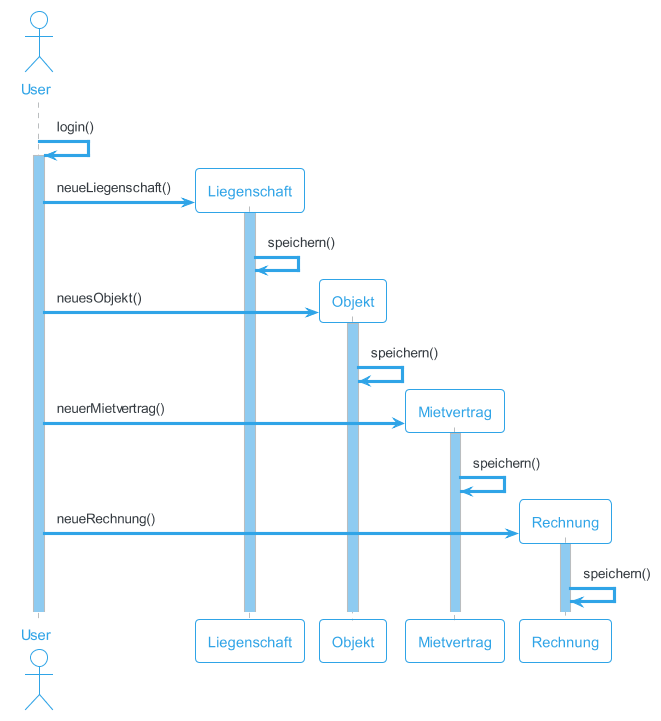
\includegraphics[width=1\linewidth]{content/diagrams/out/sequenzdiagram/sequenzdiagram.png}
    \caption{Sequenzdiagramm}
    \label{sequenzdiagram}
  \end{center}
\end{figure}

\newpage
\subsection{Modellierung der Klassen}
\subsubsection{Klassendiagramm}
\begin{figure}[htbt]
  \begin{center}
    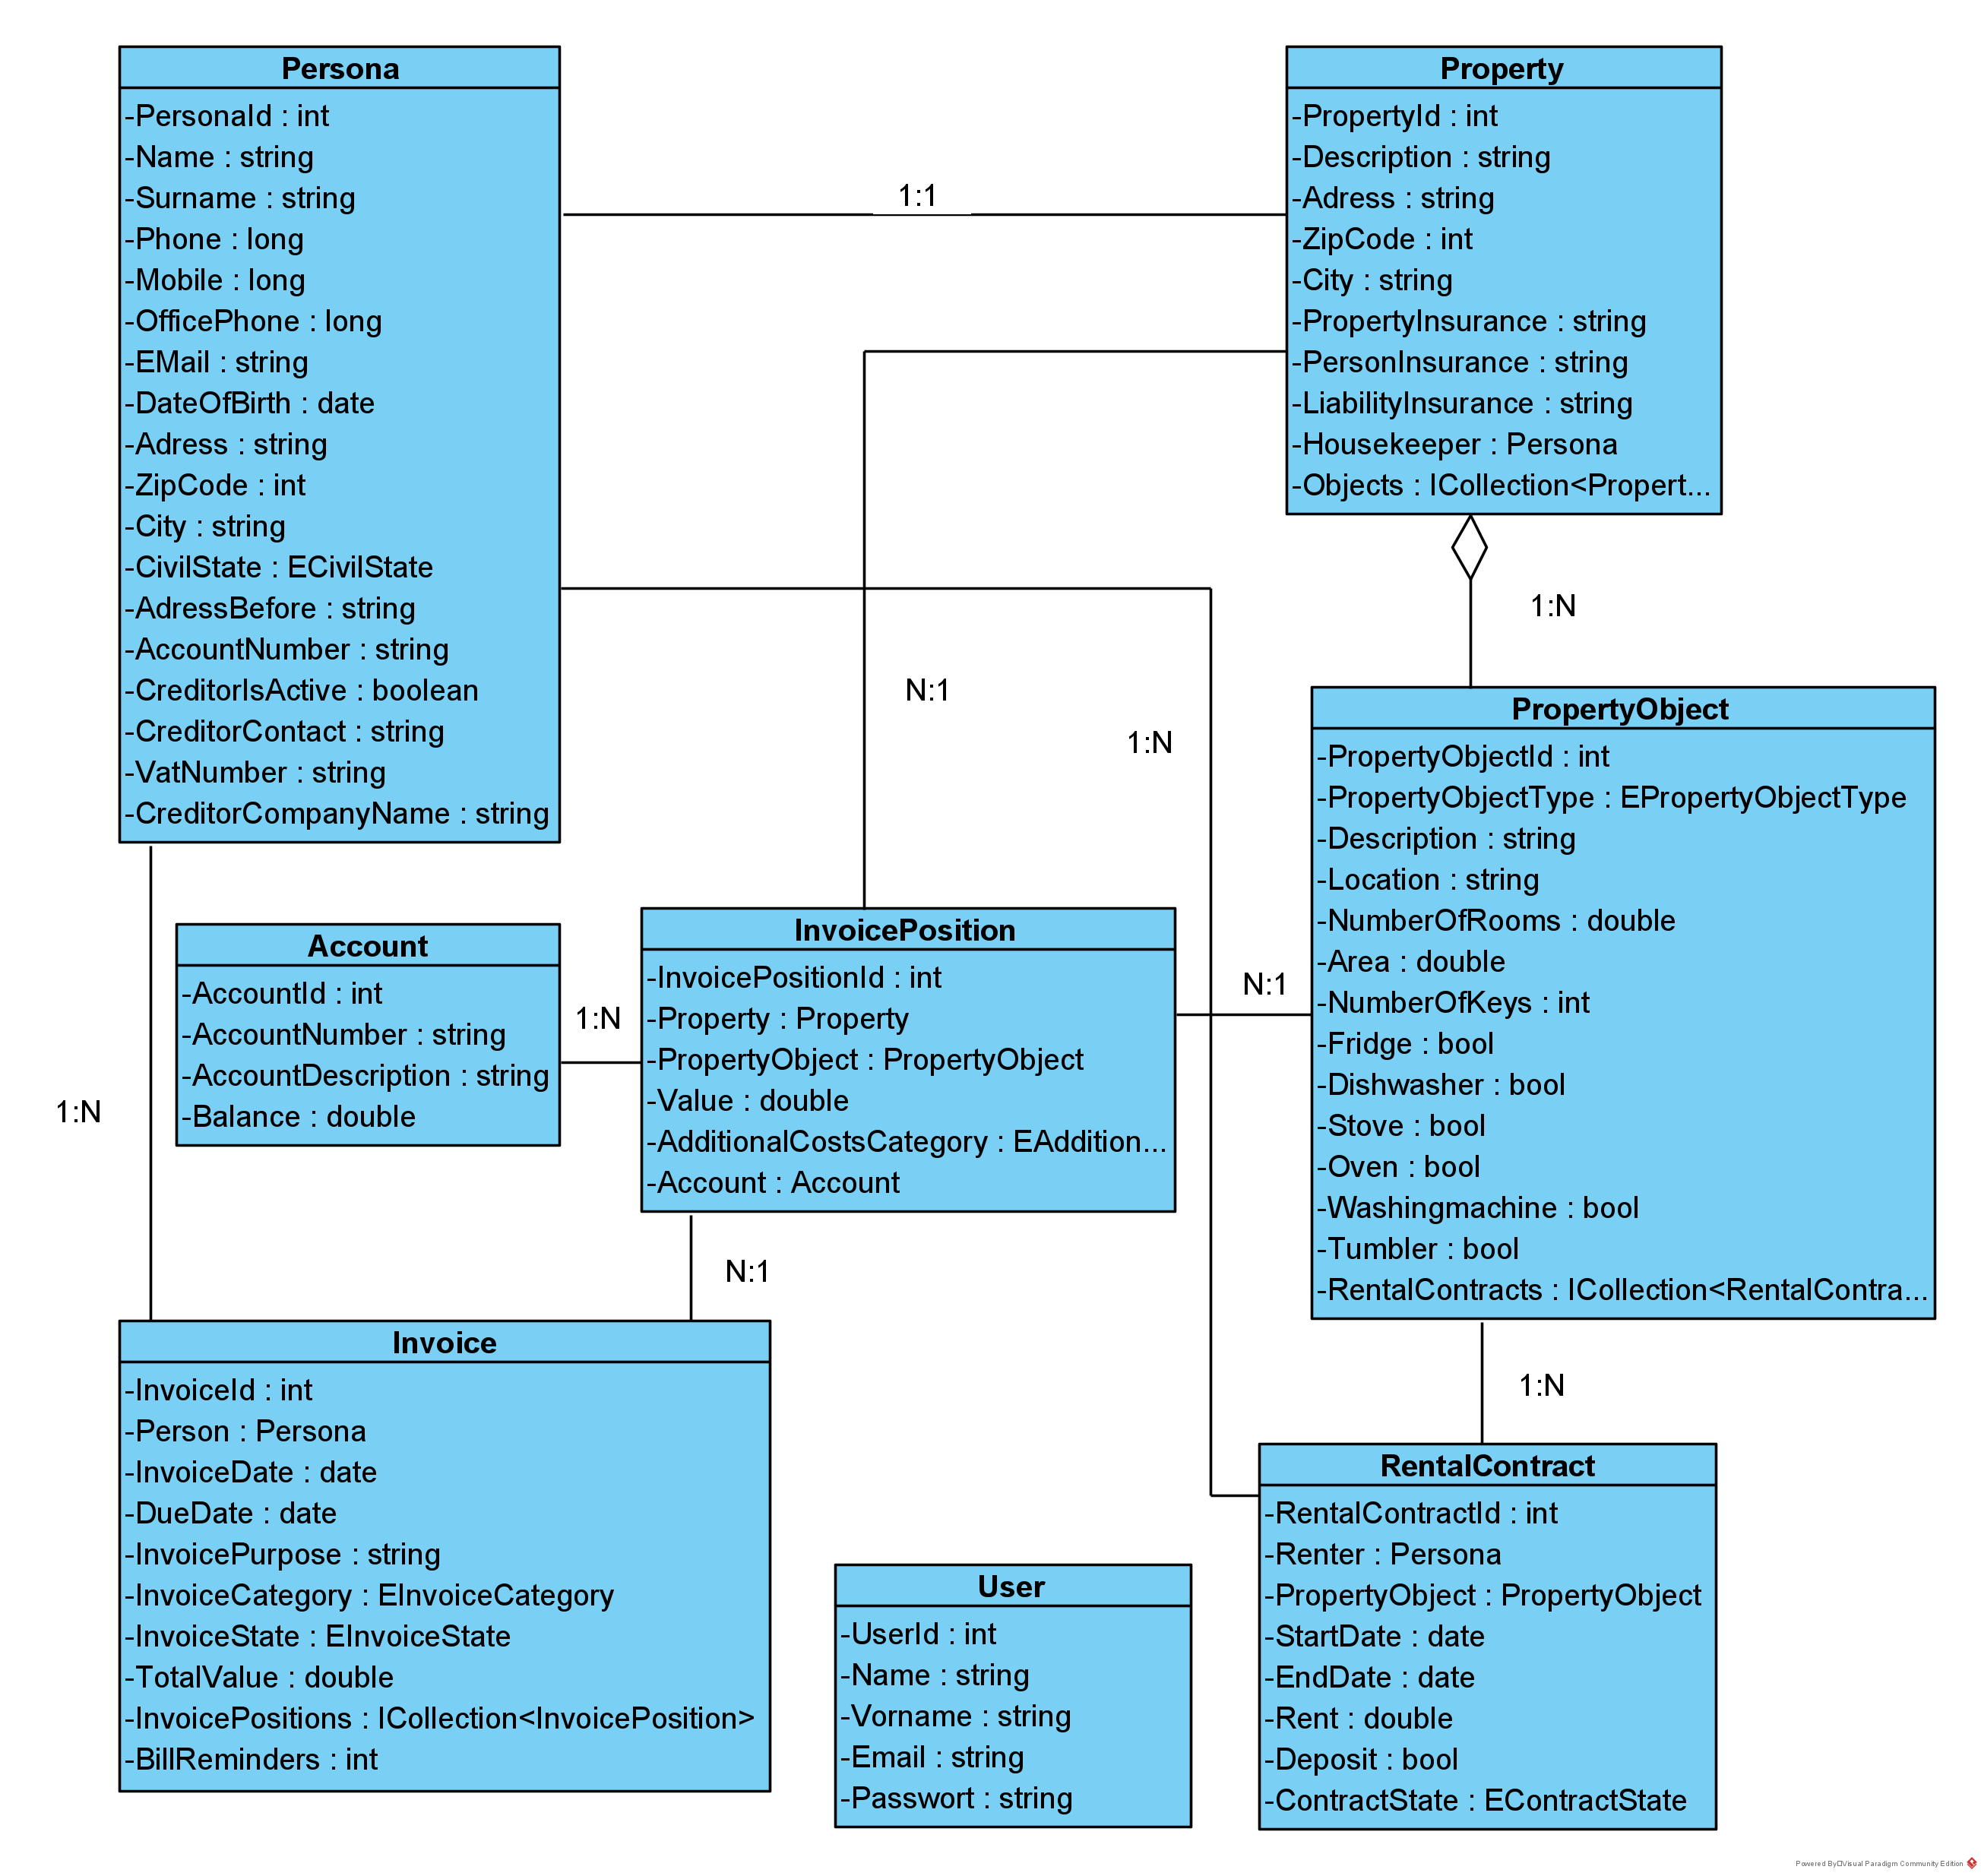
\includegraphics[width=0.9\linewidth]{content/diagrams/out/classdiagram/classdiagram.png}
    \caption{Klassendiagramm}
    \label{classdiagramm}
  \end{center}
\end{figure}

\subsubsection{Beschreibung der Fachklassen}
\begin{table}[H]
  \centering
  \settowidth\tymin{\textbf{Liegenschaft}}
  \setlength\extrarowheight{2pt}
    \begin{tabulary}{1.0\textwidth}{|L|m{15cm}|}
      \hline
      \rowcolor[HTML]{4473C5}\textbf{Klasse}& \textbf{Beschreibung}\\
    \hline
    \textbf{Persona} & Bildet alle Beteiligten Personen ab. Es werden die Mieter:in, Kreditor und die Hauswartungsperson über diese Klasse erfasst. Z.B. für den Mieter:in werden nicht alle Eigenschaften verwendet, wie auch für den Kreditor oder die Hauswartungsperson nicht alle Eigenschaften verwendet werden. Für jede Personengruppe wird ein separater Konstruktor erstellt.\\
    \hline
    \textbf{Liegenschaft} & Bildet die Liegenschaft mit ihren Eigenschaften ab und beinhaltet die Hauswartungsperson als Persona Objekt. Jede Liegenschaft kann N-Objekte enthalten.\\
    \hline
    \textbf{Objekt} & Bildet das Objekt, welches in der Liegenschaft enthalten ist, mit seinen Eigenschaften ab. Jedes Objekt kann nur Eine Beziehungen zu einer Liegenschaft haben. Pro Objekt können aber N-Mietverträge vorhanden sein, wobei immer nur einer gültig sein darf. \\
    \hline
    \textbf{Mietvertrag} & Bildet den Mietvertrag mit seinen Eigenschaften ab. Jeder Mietvertrag kann einem Objekt zugeordnet sein. Der Mietvertrag ist entweder gültig oder ungültig.\\
    \hline
    \textbf{Rechnung} & Bildet die Rechnung mit ihren Eigenschaften ab. Es kann eine Rechnung auf ein Objekt oder auf eine Liegenschaft erstellt werden und einem Mieter oder einem Kreditor über ''Persona'' zugeordnet werden.\\
    \hline
    \textbf{User} & Bildet die User für das Login in der Applikation ab.\\
    \hline
    \textbf{Konto} & Bildet das Konto zum Verbuchen der Rechnung ab.\\
    \hline 
\end{tabulary}
\caption{Beschreibung der Fachklassen}
\end{table}

\subsection{Zustandsdiagramme}
\begin{figure}[H]
  \begin{center}
    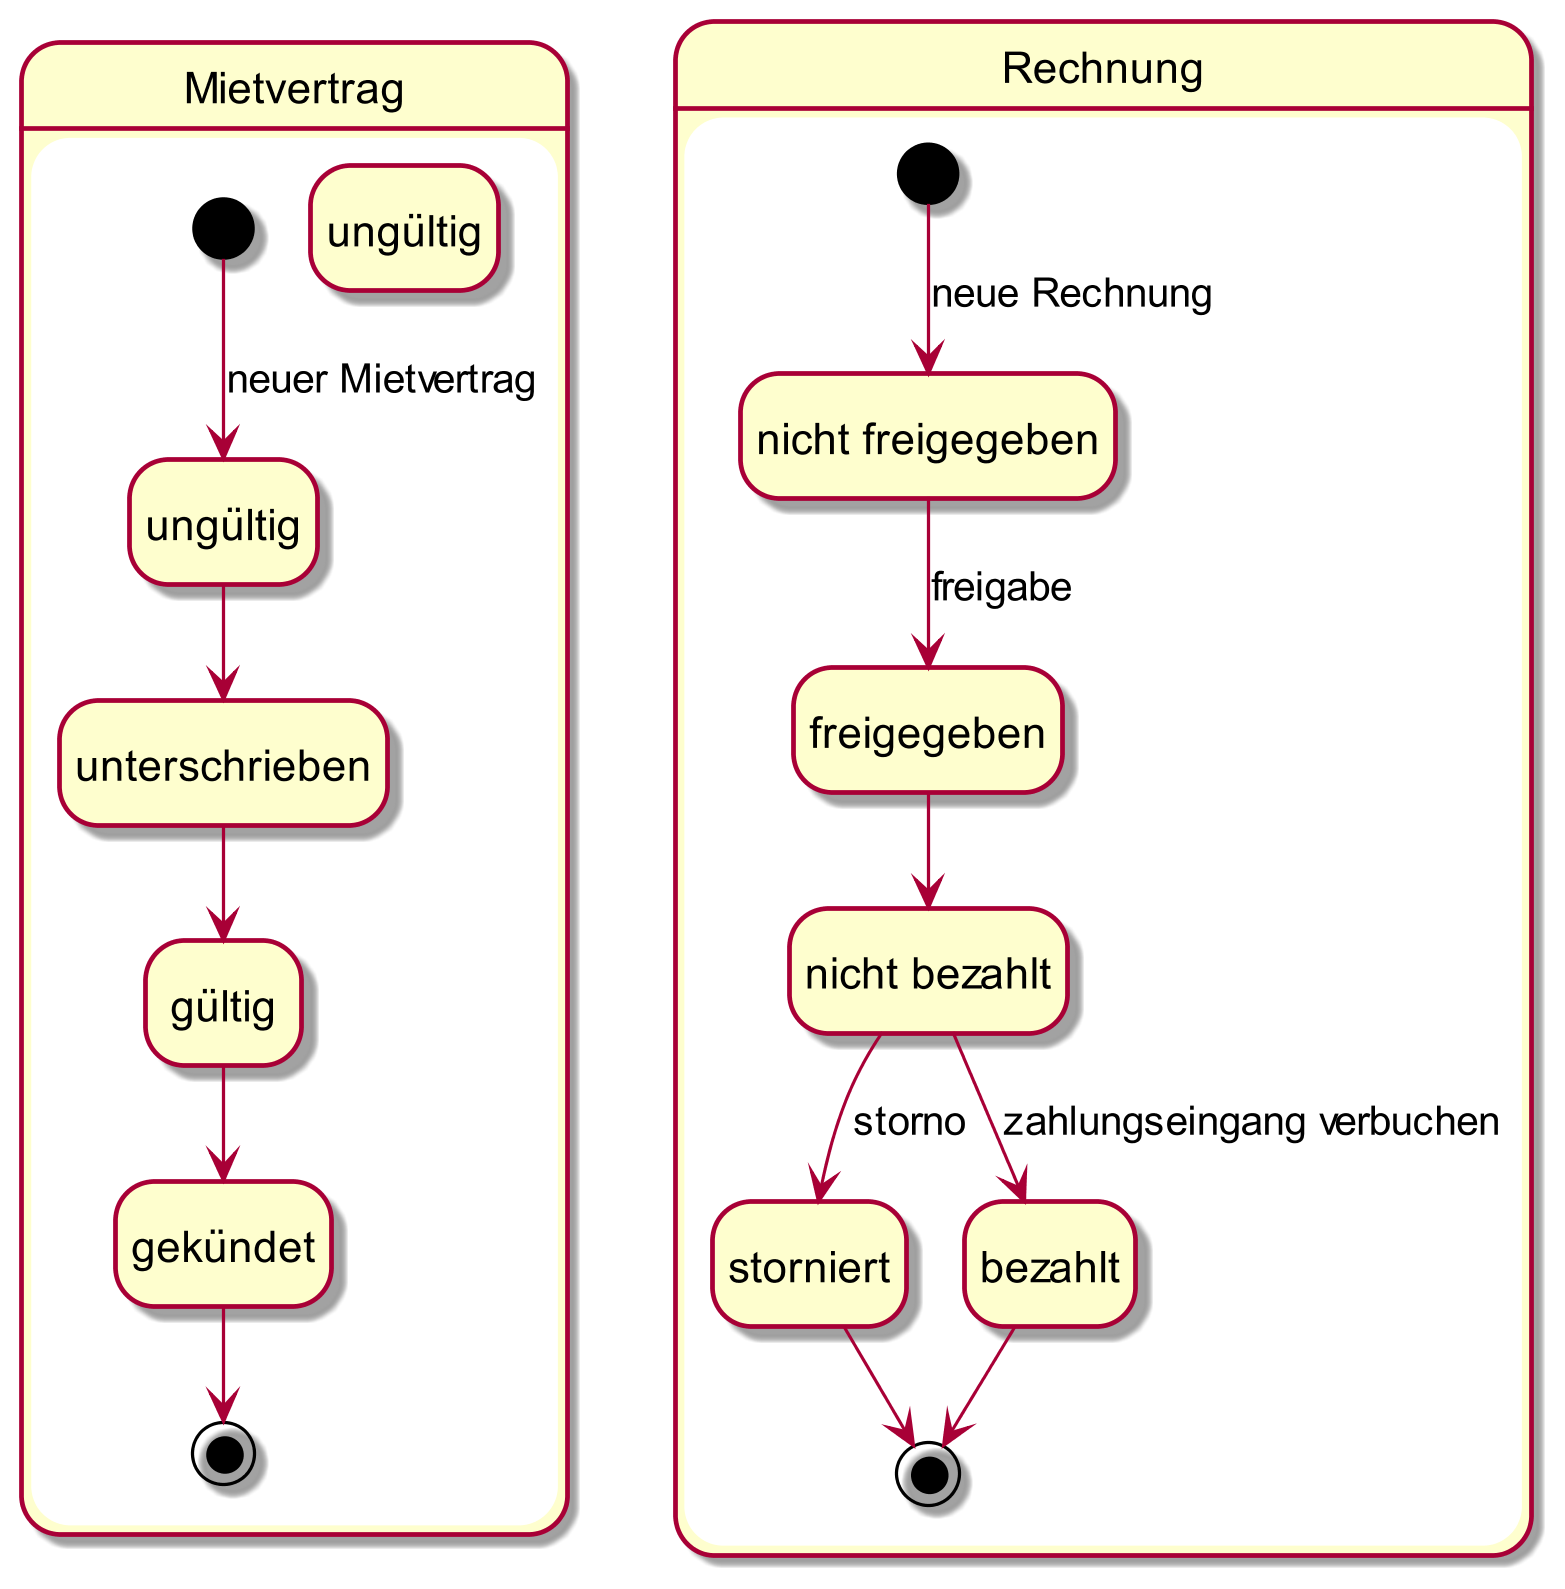
\includegraphics[height=0.6\textheight]{content/diagrams/out/zustand/mietvertragRechnung/mietvertragRechnung.png}
    \caption{Zustand Mietvertrag}
    \label{zustMietvertrag}
  \end{center}
\end{figure}

\subsection{Modellierung der Datenbank}

\subsubsection{ERD}
\begin{figure}[H]
  \begin{center}
    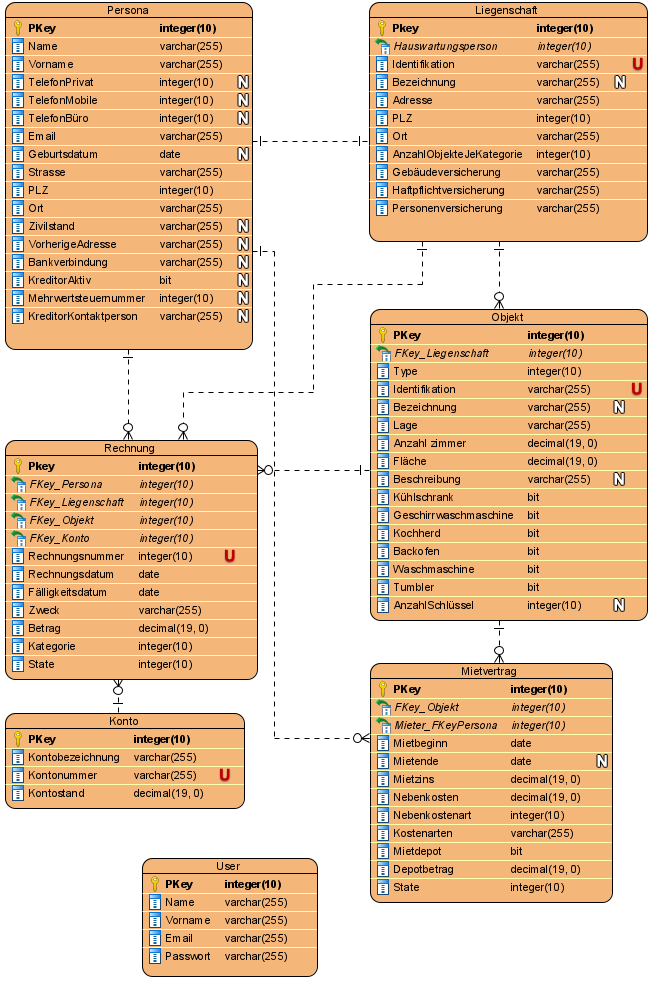
\includegraphics[height=0.85\textheight]{content/diagrams/out/erd/erd.png}
    \caption{ERD}
    \label{ERD}
  \end{center}
\end{figure}

\subsubsection{Beschreibung der Fachentitäten}
\begin{table}[H]
  \centering
  \settowidth\tymin{\textbf{Liegenschaft}}
  \setlength\extrarowheight{2pt}
    \begin{tabulary}{1.0\textwidth}{|L|m{15cm}|}
      \hline
      \rowcolor[HTML]{4473C5}\textbf{Entität}& \textbf{Beschreibung}\\
    \hline
    \textbf{Liegenschaft} & Bildet die Liegenschaft ab. Hat eine 1:N Beziehungen zur Objekt- und zur Rechnungsentität.\\
    \hline
    \textbf{Objekt} & Bildet das Objekt ab. Das Objekt hate eine N:1 Beziehung zur Liegenschaft, beinhaltet also dessen Foreign-Key. Zusätzlich hat das Objekt noch eine 1:N-Beziehung zur Rechnung.\\
    \hline
    \textbf{Mietvertrag} & Bildet den Mietvertrag ab. Diese Entität beinhaltet den Foreign-Key von der Entität Persona zum Referenzieren des Mieters und den Foreign-Key zum Objekt, auf welches der Mietvertrag läuft. \\
    \hline
    \textbf{Persona} & Bildet alle Beteiligten Personen ab. Es werden die Mieter:in, Kreditor und die Hauswartungsperson über diese Entität erfasst. Somit ist je ein Foreign-Key in der Rechnung und im Mietvertrag enthalten. \\
    \hline
    \textbf{Rechnung} & Bildet die Rechnung ab. Da die Rechnung zur Liegenschaft und zum Objekt gestellt werden muss, ist je ein Foreign-Key von diesen Entitäten enthalten. Zum Verbuchen auf ein Konto wir der Foreign-Key der Entität Konto verwendet. Damit die Rechnung einem Mieter oder Kreditor gestellt werden kann, wird der Foreign-Key Persona verwendet.\\
    \hline
    \textbf{Konto} & Bildet das Konto zum Verbuchen der Rechnung ab und hat somit eine 1:N-Beziehung zur Rechnung\\
    \hline
    \textbf{User} & Bildet die User für das Login in der Applikation ab. Das Passwort wird als HASH gespeichert.\\
    \hline 
\end{tabulary}
\caption{Beschreibung der Fachentitäten}
\end{table}

\subsection{Systemarchitektur}
Die Programmiersprache für die Applikation ist C\# mit dem aktuellen .net Core 6 Framework. Das GUI wird mit WPF aufgebaut und die gesamte Struktur im MVVM-Pattern gehalten. Mit WPF werden alle GUI-Komponenten über Binding angesteuert, was es in einem weiteren schritt viel einfacher mach die Applikation mehrsprachig zu gestalten.\\ Um das GUI ansprechend zu gestalten, wird das NuGet-Paket ''Material-Design'' und das Font Awesome Paket verwendet.\\
Für das persistieren der Daten wird das ORM Entity-Framework benutzt, mit welchem bereits in einem früheren Projekt Erfahrungen gesammelt werden konnten.

\newpage
\subsection{Testkonzept} \label{testkonzept}
\subsubsection{Vorgehen}
Anhand von Szenarien die aus den Use-Case's erstellt werden und dann nach ihrer Eintrittswahrscheinlichkeit und dem Ausmass bewertet werden, werden die Testfälle gebildet. Das Risiko leitet sich aus der Multiplikation der Eintrittswahrscheinlichkeit und dem Ausmass ab.
\subsubsection{Testobjekte}
\begin{table}[H]
  \centering
  \setlength\extrarowheight{2pt}
  \begin{tabulary}{1.0\textwidth}{LCL}
    \textbf{Eintrittswahrscheinlichkeit (ETW)} & &
    \textbf{Ausmass (Ausm.)} \\
    1 = Sehr unwahrscheinlich\newline  2 = Unwahrscheinlich\newline 3 = Möglich\newline 4 = Gelegentlich\newline 5 = Häufig && 1 = Kaum bemerkbar\newline 2 = Bemerkbar \newline 3 = Störend \newline 4 = Stark störend \newline 5 = Katastrophal\\
  \end{tabulary}
\end{table}

\begin{table}[H]
  \centering
  \settowidth\tymin{\textbf{Mietverträge}}
  \setlength\extrarowheight{2pt}
  \begin{tabulary}{1.0\textwidth}{|L|L|L|C|C|C|}
    \hline
    \rowcolor[HTML]{fdebd0}
    \textbf{UseCase} & 
    \textbf{Positiv}& 
    \textbf{Negativ} &
    \textbf{ETW} & 
    \textbf{Ausm.} & 
    \textbf{Risiko}\\
    \hline
    Login & \cellcolor[HTML]{02ce16} Der User kann sich mit korrekten Logindaten einloggen & \cellcolor[HTML]{ff0000}$\bullet$ Der User kann sich nur mit Username einloggen \newline $\bullet$  Der User kann sich mit einem falschen Passwort einloggen & 3 & 5 & \cellcolor[HTML]{ff8c00} 15\\
    \hline
    Liegenschaft erfassen & \cellcolor[HTML]{02ce16} Der User kann die Liegenschaft abspeichern, wenn alle Muss-Daten eingegeben wurden & \cellcolor[HTML]{ff0000}$\bullet$ Der User kann die Liegenschaft nicht abspeichern, wenn alle Muss-Daten eingegeben wurden \newline $\bullet$  Der User kann die Liegenschaft abspeichern, obwohl nicht alle Muss-Daten eingegeben wurden  & 3 & 4 & \cellcolor[HTML]{ffb600} 12\\
    \hline
    Objekt erfassen & \cellcolor[HTML]{02ce16} Der User kann das Objekt abspeichern, wenn alle Muss-Daten eingegeben wurden & \cellcolor[HTML]{ff0000}$\bullet$ Der User kann das Objekt nicht abspeichern, wenn alle Muss-Daten eingegeben wurden \newline $\bullet$  Der User kann das Objekt abspeichern, obwohl nicht alle Muss-Daten eingegeben wurden & 3 & 4 & \cellcolor[HTML]{ffb600} 12\\
    \hline
    Mietverträge verwalten & \cellcolor[HTML]{02ce16} Der User kann einen neuen Mietvertrag erstellen, wenn alle Muss-Daten eingegeben wurden & \cellcolor[HTML]{ff0000}$\bullet$ Der User kann den Mietvertrag nicht erstellen, obwohl alle Muss-Daten eingegeben wurden \newline $\bullet$  Der User kann den Mietvertrag erstellen, obwohl nicht alle Muss-Daten eingegeben wurden & 3 & 4 & \cellcolor[HTML]{ffb600} 12\\
    \hline
    Mietverträge verwalten & \cellcolor[HTML]{02ce16} Der User kann den Status eines bestehenden Mietvertrages von ungültig auf gültig bzw. von gültig auf ungültig ändern & \cellcolor[HTML]{ff0000}$\bullet$ Der Status des Mietvertrages kann nicht auf gültig bzw. ungültig geändert werden & 3 & 4 & \cellcolor[HTML]{ffb600} 12\\
    \hline
  \end{tabulary}
  \caption{Testfallanalyse (1)}
  \label{testanforderungen}
\end{table}


\begin{table}[H]
  \centering
  \settowidth\tymin{\textbf{Mietverträge}}
  \setlength\extrarowheight{2pt}
  \begin{tabulary}{1.0\textwidth}{|L|L|L|C|C|C|}
    \hline
    \rowcolor[HTML]{fdebd0}
    \textbf{UseCase} & 
    \textbf{Positiv}& 
    \textbf{Negativ} &
    \textbf{ETW} & 
    \textbf{Ausm.} & 
    \textbf{Risiko}\\
    \hline
    Mietzins-kontrolle & \cellcolor[HTML]{02ce16} Der User kann das betreffende Objekt auswählen und der aktuelle Mietzins \& die Nebenkosten werden angezeigt & \cellcolor[HTML]{ff0000}$\bullet$ Es werden keine Objekte angezeigt \newline $\bullet$  Nach dem anwählen des Objektes, werden die falschen Daten geladen \newline $\bullet$ Nach dem anwählen des Objektes werden keine Daten geladen & 3 & 4 & \cellcolor[HTML]{ffb600} 12\\
    \hline
    Mahnung erstellen & \cellcolor[HTML]{02ce16} Der User kann den Mieter/Kreditor zum erstellen der Mahnung auswählen und die Mahnung anschliessend generieren. Auf der Mahnung sind alle Daten korrekt eingetragen & \cellcolor[HTML]{ff0000}$\bullet$ Der Mieter/Kreditor kann nicht ausgewählt werden \newline $\bullet$ Es werden die falschen Daten in die Mahnung eingefügt & 3 & 4 & \cellcolor[HTML]{ffb600} 12\\
    \hline
    Rechnung erstellen & \cellcolor[HTML]{02ce16} Der User kann alle relevanten Daten für die Rechnung auswählen. Die Rechnung wird mit den korrekten Daten generiert und kann ausgedruckt werden. Die Rechnung kann nur generiert werden, wenn alle Muss-Daten ausgefüllt wurden & \cellcolor[HTML]{ff0000}$\bullet$ Der Kreditor/Mieter kann nicht ausgewählt werden \newline $\bullet$ Das Konto für die Einzahlung kann nicht ausgewählt werden \newline $\bullet$ Es kann keine Kategorie ausgewählt werden \newline $\bullet$ Die Rechnung kann erstellt werden, obwohl nicht alle Muss-Daten eingegeben wurden & 4 & 4 & \cellcolor[HTML]{ff8c00} 16\\
    \hline
    Kreditor erfassen & \cellcolor[HTML]{02ce16} Der User kann den Kreditor nach Eingabe aller Muss-Daten erfolgreich abspeichern & \cellcolor[HTML]{ff0000}$\bullet$ Der Kreditor kann abgespeichert werden, obwohl nicht alle Muss-Daten eingegeben wurden \newline $\bullet$ Der Kreditor kann nicht abgespeichert werden obwohl alle Muss-Daten eingegeben wurden & 3 & 4 & \cellcolor[HTML]{ffb600} 12\\
    \hline
    Mieter erfassen & \cellcolor[HTML]{02ce16} Der User kann den Mieter nach Eingabe aller Muss-Daten erfolgreich abspeichern & \cellcolor[HTML]{ff0000}$\bullet$ Der Mieter kann abgespeichert werden, obwohl nicht alle Muss-Daten eingegeben wurden \newline $\bullet$ Der Mieter kann nicht abgespeichert werden, obwohl alle Muss-Daten eingegeben wurden & 3 & 4 & \cellcolor[HTML]{ffb600} 12\\
    \hline
  \end{tabulary}
  \caption{Testfallanalyse (2)}
  \label{testanforderungen2}
\end{table}

\subsubsection{Testfälle}

\begin{table}[H]
  \centering
  \settowidth\tymin{\textbf{Mietverträge}}
  \setlength\extrarowheight{2pt}
  \begin{tabulary}{1.0\textwidth}{|L|L|L|L|}
    \hline
    \rowcolor[HTML]{fdebd0}
    \textbf{UseCase} & 
    \textbf{Testfall}& 
    \textbf{Soll} &
    \textbf{Wichtigkeit}\\
    \hline
    Login & In 10 Loginversuchen haben 3 ein Falsches Passwort und 3 kein Passwort & Alle 6 ungültigen Loginversuche werden erkannt, die 4 korrekten Loginversuche werden korrekt eingeloggt & Critical\\
    \hline
    Liegenschaft erfassen & In 10 zu erfassenden Liegenschaften werden 3 Datensätze verwendet die nicht alle Muss-Daten enthalten & Die 7 korrekten Datensätze werden erfolgreich abgespeichert und die 3 ungültigen Datensätze werden mit einer Fehlermeldung abgewiesen & Critical\\
    \hline
    Liegenschaft erfassen & In 10 zu erfassenden Liegenschaften werden 3 Datensätze verwendet die nicht alle Muss-Daten enthalten & Die 7 korrekten Datensätze werden erfolgreich abgespeichert und die 3 ungültigen Datensätze werden mit einer Fehlermeldung abgewiesen & Critical\\
    \hline
    Objekt erfassen & In 10 zu erfassenden Objekten werden 3 Datensätze verwendet die nicht alle Muss-Daten enthalten & Die 7 korrekten Datensätze werden erfolgreich abgespeichert und die 3 ungültigen Datensätze werden mit einer Fehlermeldung abgewiesen & Critical\\
    \hline
    Mietverträge verwalten & In 10 zu erfassenden Mietverträgen werden 3 Datensätze verwendet die nicht alle Muss-Daten enthalten & Die 7 korrekten Datensätze werden erfolgreich abgespeichert und die 3 ungültigen Datensätze werden mit einer Fehlermeldung abgewiesen & Critical\\
    \hline
    Mietverträge verwalten & Es werden bei 10 Mietverträgen die Stati von ungültig zu gültig verändert und gespeichert & Bei allen 10 Mietverträgen wird der Status gültig gespeichert & Critical\\
    \hline
    Mietverträge verwalten & Es werden bei 10 Mietverträgen die Stati von gültig zu ungültig verändert und gespeichert & Bei allen 10 Mietverträgen wird der Status ungültig gespeichert & Critical\\
    \hline
    Mietzins-kontrolle & In einer Stichprobe werden 10 verschiedenen Objekte von unterschiedlichen Liegenschaften geladen & Es werden bei allen 10 Objekten der aktuelle und korrekte Mietzins und die korrekten Nebenkosten angezeigt & Critical\\
    \hline
    Mahnung erstellen & In einer Stichprobe werden 5 Mahnungen für Mieter und 5 Mahnungen für Kreditoren generiert & Es können alle Mahnungen mit gültigen Daten generiert werden & Critical\\
    \hline
  \end{tabulary}
  \caption{Testfälle (1)}
  \label{Testfälle1}
\end{table}

\begin{table}[H]
  \centering
  \settowidth\tymin{\textbf{Mietverträge}}
  \setlength\extrarowheight{2pt}
  \begin{tabulary}{1.0\textwidth}{|L|L|L|L|}
    \hline
    \rowcolor[HTML]{fdebd0}
    \textbf{UseCase} & 
    \textbf{Testfall}& 
    \textbf{Soll} &
    \textbf{Wichtigkeit}\\
    \hline 
    Rechnung erstellen & Es werden 10 Rechnungen erstellt. Für 3 Rechnungen werden nicht alle Muss-Daten angegeben & Die 7 gültigen Rechnungen werden erfolgreich erstellt und dir 3 ungültigen werden mit einer Fehlermeldung abgewiesen & Critical\\
    \hline   
    Rechnung erstellen & In einer Stichprobe werden 5 Rechnungen für Mieter und 5 Rechnungen für Kreditoren erstellt & Es können alle Rechnungen mit gültigen Daten erstellt werden & Critical\\
    \hline
    Kreditor erfassen & Bei 10 zu erfassenden Kreditoren, werden 3 Datensätze verwendet, die nicht alle Muss-Daten enthalten & Die 7 korrekten Datensätze werden erfolgreich abgespeichert und die 3 ungültigen Datensätze werden mit einer Fehlermeldung abgewiesen & Critical\\
    \hline
    Mieter erfassen & Bei 10 zu erfassenden Mieter:innen, werden 3 Datensätze verwendet, die nicht alle Muss-Daten enthalten & Die 7 korrekten Datensätze werden erfolgreich abgespeichert und die 3 ungültigen Datensätze werden mit einer Fehlermeldung abgewiesen & Critical\\
    \hline
  \end{tabulary}
  \caption{Testfälle (2)}
  \label{Testfälle2}
\end{table}
\subsection{Einführungskonzept}
 Die Applikation wird in einem einfachen Einführungskonzept eingeführt. Nach dem vorstellen des Prototypen wird die Applikation nach dem Kundenfeedback angepasst und evtl. die Funktionalität erweitert. Sobald die Applikation dann soweit ist dass sie vom Kunden benutzt werden kann, wird sie installiert damit die Mitarbeiter beginnen können die Applikation zu nutzen die Funktionalität zu testen und die Daten zu erfassen. Während diesem Prozess müssen allfällige Fehler sofort behoben werden was einen engen Kundenkontakt während der Einführungszeit erfordert. 

\subsection{GUI Konzept}
\subsubsection{GUI-Map}
\vspace*{-1cm}
\begin{figure}[H]
  \begin{center}
    \includegraphics[height=0.9\textheight]{content/diagrams/out/guiMap/GuiMindMap.png}
    \caption{GUI-Map}
    \label{guiMap}
  \end{center}
\end{figure}
\subsubsection{GUI-Map Beschreibung}
Über die Liegenschaft gelangt der User zum Objekt oder er kann sich direkt die zuständige Hauswartungsperson anzeigen lassen, sie editieren oder neu hinzufügen. Über das Objekt können anschliessend die Mieter und die Mietverträge mit den dazugehörigen Rechnungen angesehen, bzw. editiert oder neu erstellt werden.\\
Über die Kreditoren können die dazugehörigen Rechnungen angesehen oder neu erstellt werden. \\ 
Über den Mieter können die vom Mieter gemieteten Objekte, seine Rechnungen und die Mietverträge angesehen, bzw. bearbeitet werden oder es kann ein neuer Mieter erstellt werden.\\
Wie im Geschäftsanwendungsfall \textbf{\hyperref[GA-rechnungErstellen]{Rechnung Erstellen}}  beschrieben, kann eine schon freigegebene Rechnung nicht mehr verändert werden.\\
Über die Rechnung kann eine neue Rechnung erstellt werden. Es kann dann ausgewählt werden für welches Objekt, Liegenschaft, Kreditor oder Mieter die Rechnung erstellt werden soll.\\
Über das Konto hat der Benutzer die Möglichkeit die Zahlungen zu verbuchen oder ein neues Konto zu erstellen.\\

\subsubsection{GUI Design}
\foreach \x in {1,...,20}
{ 
  \edef\FileName{content/images/GUI-Design/Folie\x.PNG}%
  \IfFileExists{\FileName}{%
     \begin{figure}[H] %
       \begin{center}%
         \includegraphics[height=0.65\textwidth]{\FileName}%
         \caption{GUI Design Screen \x}%
         \label{guiDesignScreen\x}%%
       \end{center}%
     \end{figure}%
     \vspace*{-1cm}%
  }
}